\chapter{Fejlesztői dokumentáció}
\label{ch:impl}

\section{Fejlesztői környezet}

\subsection{Szükséges szoftver}

\begin{itemize}
    \item git
    \item Windows 10 20H2 (2020 Októberi frissítés) vagy újabb.
    \item Visual Studio 2022
    \item Windows 10 SDK 2004-es verzió
    \item NVIDIA GPU driver 466.11, vagy újabb
\end{itemize}

\subsection{Környezet előkészítése}

A program egy Falcor alkalmazás, ezért mindenek előtt szükségünk van a keretrendszer forráskódjára. A fejlesztéshez az 5.2-es verzióra van szükségünk, ezért át kell váltanunk az 5.2-es címkével ellátott állapotra.

\lstset{caption={Falcor 5.2 forráskód letöltése git segítségével}, label=src:falcor-clone}
\begin{lstlisting}[language=bash]
	git clone https://github.com/NVIDIAGameWorks/Falcor.git
	cd Falcor
	git checkout tags/5.2
\end{lstlisting}

Az alkalmazás a keretrendszer részeként egyszerűen lefordítható a keretrendszerrel mellékelt scriptekkel, ezért másoljuk be a szakdolgozat forráskódját a \textit{Falcor/Source/Samples/} mappába, majd adjuk hozzá a mappát a \textit{Falcor/Source/Samples/CMakeLists.txt} fájlhoz a következő módon:
\lstset{caption={PolygonSDF hozzáadása a CMakeLists.txt-hez}, label=src:falcor-cmake}
\begin{lstlisting}
	# ... other subdirectories
	add_subdirectory(PolygonSDF)
\end{lstlisting}

Miután kész a mappastruktúra a fejlesztéshez, a build rendszer segítségével le kell generálnunk a Visual Studio projektfájlokat. Szerencsére a keretrendszer készítői gondoskodtak arról, hogy ez a lépés a lehet legegyszerűbb legyen, a \textit{Falcor/setup\_vs2022.bat} batch fájl végrehajtásával minden előkészítésre kerül.


\subsection{Az alkalmazás projektjei}

Nyissuk meg Visual Studio-ban a \textit{Falcor/build/windows-vs2022-d3d12/Falcor.sln} fájlt! A szakdolgozat négy projektből áll, melyeket a \textit{Solution Explorer > [Project] > Set as Startup Project} beállítása után az indítás gombbal fordíthatunk:

\begin{figure}[H]
    \centering
    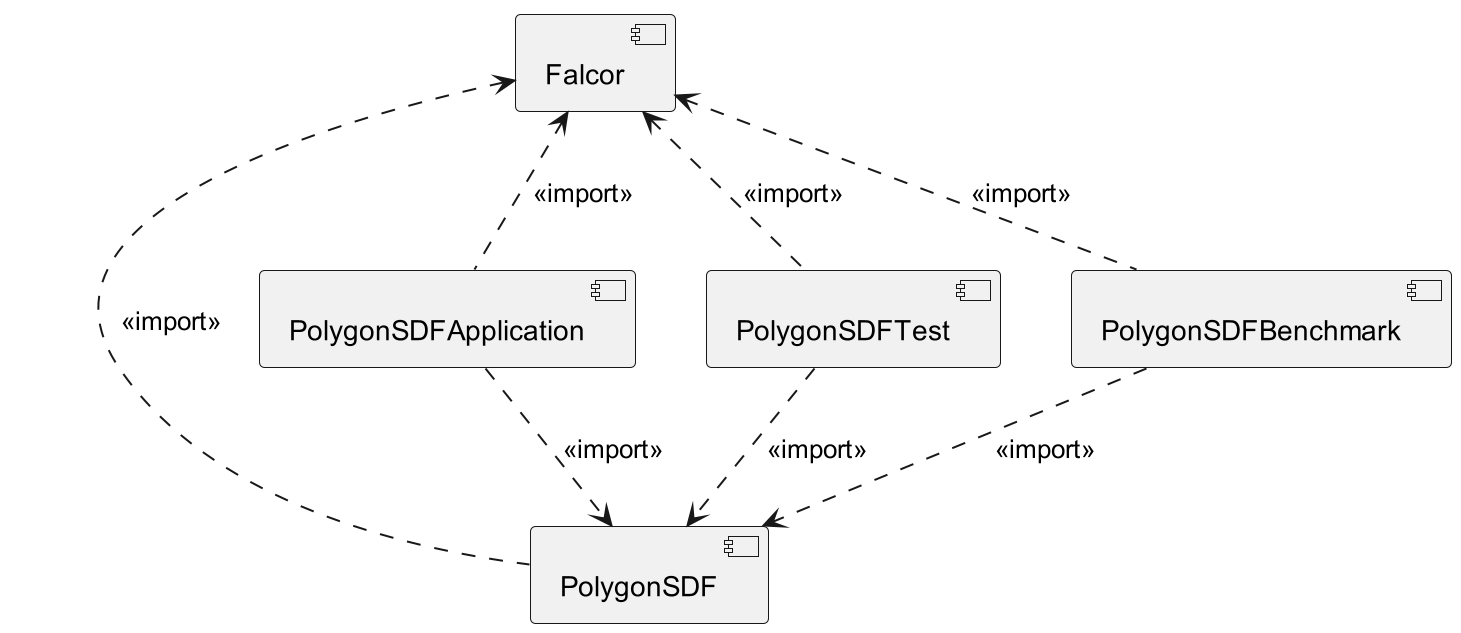
\includegraphics[width=1\linewidth]{images/component_project.png}
    \caption{Az alkalmazás csomagdiagramja}
    \label{fig:component_project-1}
\end{figure}

\begin{description}
    \item[PolygonSDF] Tartalmazza algoritmus implementációt és a szerkesztői osztályokat. Ez a projekt nem futtatható, mert egy könyvtár a fordítási folyamat eredménye.
    \item[PolygonSDFApplication] A szerkesztői osztályokat egy alkalmazásba csomagolja, itt történik azon objektumok példányosítása, melyek az alkalmazás teljes élettartamán keresztül memóriában maradnak, mint például a központi szerkesztő objektum és a felhasználói felületei. Ez a réteg  kapja meg a felhasználói bemenetet és adja tovább a szerkesztő felé.
    \item[PolygonSDFTest] Az algoritmus és szerkesztő tesztelésére szánt projekt.
    \item[PolygonSDFBenchmark] Az algoritmus teljesítményének mérésére szánt projekt.
\end{description}


\section{Algoritmus bemutatása}

\begin{definition}
    Egy ponthalmaz egy elemének a Voronoj-cellája a sík egy olyan régiója, amiben minden pont a ponthalmazból a cellához tartozó ponthoz van legközelebb.
\end{definition}

\begin{definition}
    A Voronoj-diagram a sík egy olyan felosztása amiben egy ponthalmaz minden eleméhez egy Voronoj-cellát rendelünk.
\end{definition}

A szakdolgozat keretein belül egy olyan algoritmus került implementálásra, ami egy kétdimenziós sokszöget feloszt Voronoj-cellákra, a magas szintű lépései az \ref{alg:algorithm}. algoritmus pszeudokódban láthatóak. Az algoritmus egy \textit{N} csúcsú alakzat esetén \textit{N} él- és \textit{N} csúcs régióra osztja fel a síkot, amivel azt teljesen lefedi. Mivel a megadott alakzat több egymásban elhelyezkedő poligonból is állhatnak, ezért az algoritmus futása előtt a pontok átrendezésre kerülnek, mert a megadási sorrend alapján kerül megállapításra a távolság előjele. A régiók véges csúcsszámú konvex poligonokkal vannak ábrázolva. Egy régiót úgy határozunk meg, hogy a kezdetben végtelenül nagy korlátokat vágásokkal az adott régióhoz tartozó Voronoj-cella korlátaihoz igazítjuk.

\begin{algorithm}[H]
    \caption{A vágásokat végző algoritmus pszeudokódja}
    \label{alg:algorithm}
    \textbf{Bemenet:} \textit{Shape shape} \\
    \textbf{Kimenet:} \textit{VertexRegion vertexRegions[M], EdgeRegion edgeRegions[M]}\\A meghatározott régióhatárok, M az alakzatban lévő csúcspontok száma.
    \begin{algorithmic}[1]
        \State reoderVertices(\textit{shape})
        \For{$outline$ : $shape$.getOutlines()}
            \For{$i$ : 0$,\ldots,outline$.size() - 1}
                \State $edge1$ = $outline$[i]
                \State $edge2$ = $outline$[(i + 1) \textbf{mod} $outline$.size()]
                \State $vertexRegion$ = initVertexRegion($edge1$, $edge2$)
                \State $vertexRegions$.add($vertexRegion$)
                \State $edgeRegion$ = initEdgeRegion($edge1$)
                \State $edgeRegions$.add($edgeRegion$)
            \EndFor
        \EndFor
        \State $vertexRegions$.cutWithVertices($vertexRegions$)
        \State $vertexRegions$.cutWithEdges($edgeRegions$)
        \State $edgeRegions$.cutWithVertices($vertexRegions$)
        \State $edgeRegions$.cutWithEdges($edgeRegions$)
        \State \textbf{return} \textit{\{vertexRegions, edgeRegions\}}
    \end{algorithmic}
\end{algorithm}

\begin{figure}[H]
    \centering
    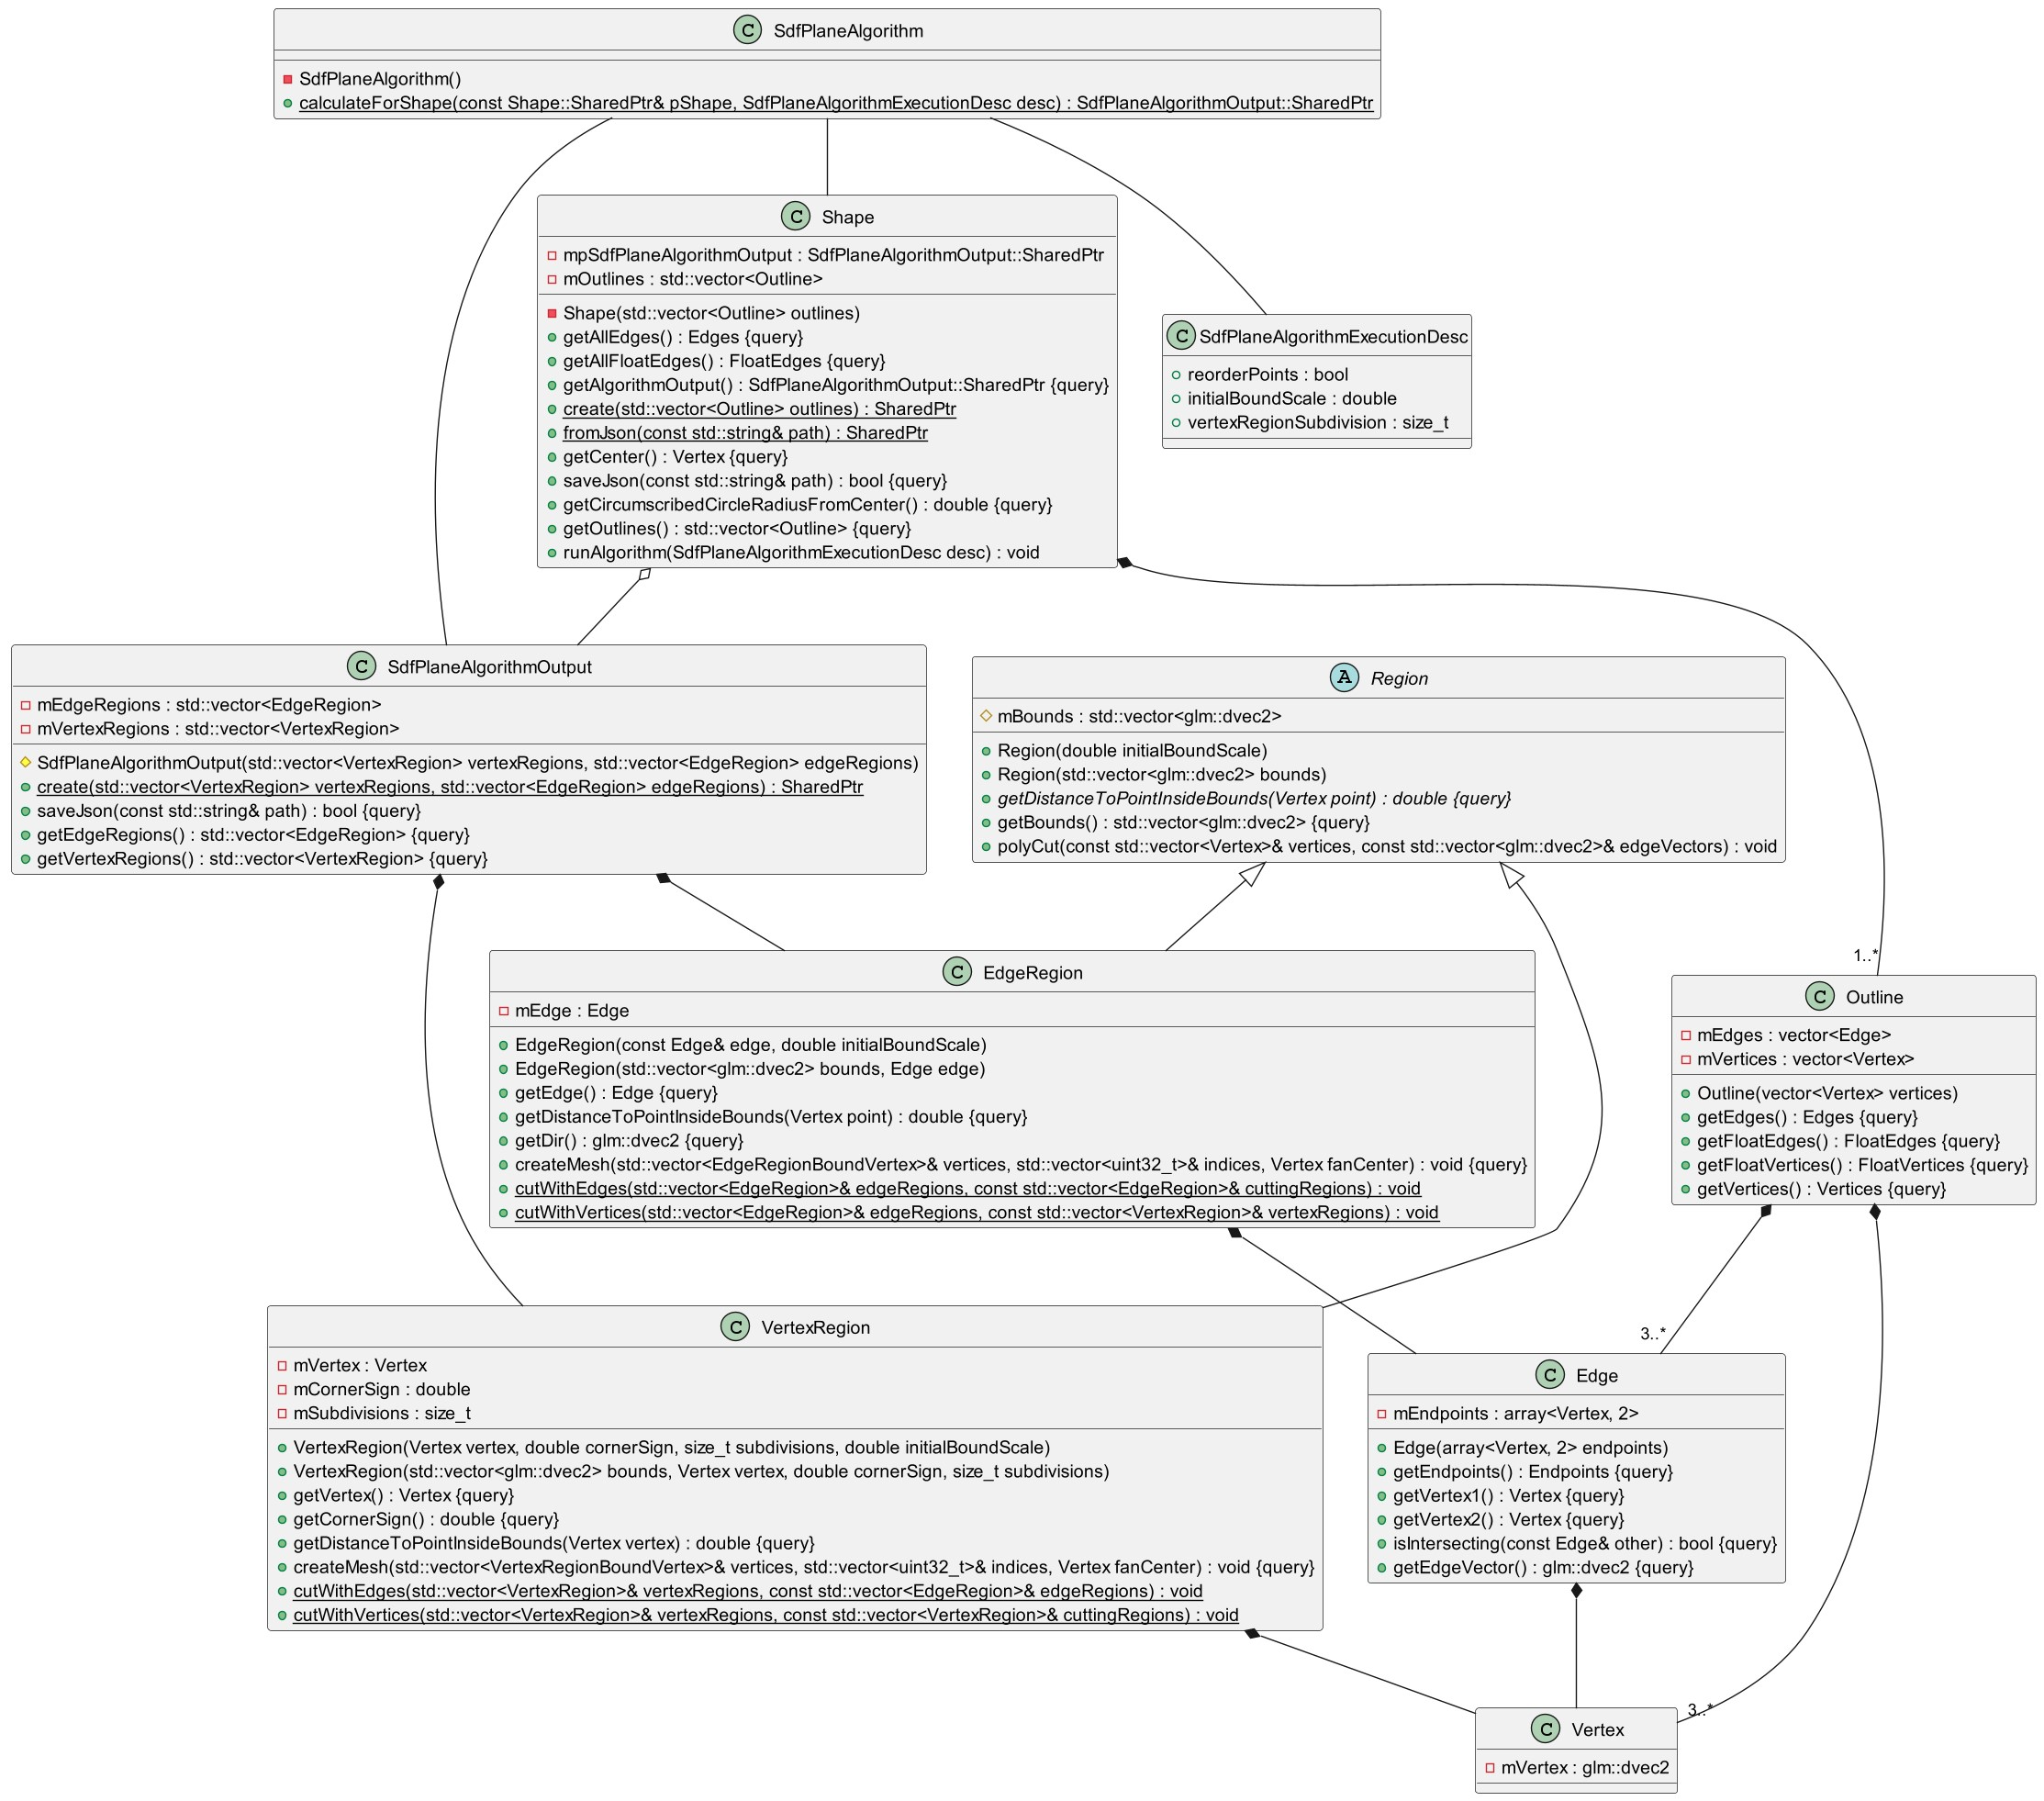
\includegraphics[width=1\linewidth]{images/class_algorithm.png}
    \caption{Az algoritmus osztálydiagramja}
    \label{fig:class_algorithm-1}
\end{figure}

\subsection{A régiók meghatározása}

A régiók vágása több lépésen keresztül történik, először felhasználjuk az információt ami az adott régió eleméhez tartozik. Csúcspontok esetén a két szomszédos él normálvektora mentén ejtünk egy-egy vágást. Élek esetében pedig a normálvektor mentén a két végponton kívül eső részt vágjuk le.

\begin{figure}[H]
    \centering
    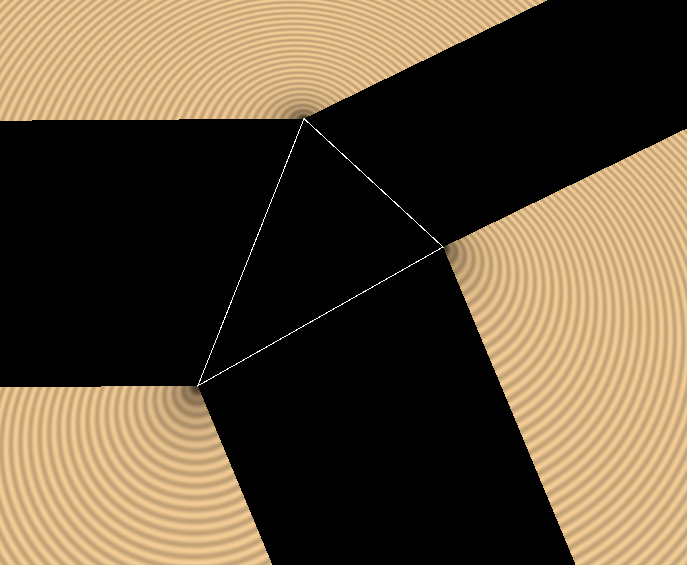
\includegraphics[width=.6\linewidth]{images/initial_vertex_regions.png}
    \caption{Csúcs régiók kezdeti határai}
    \label{fig:initial_vertex_regions-1}
\end{figure}

\begin{figure}[H]
    \centering
    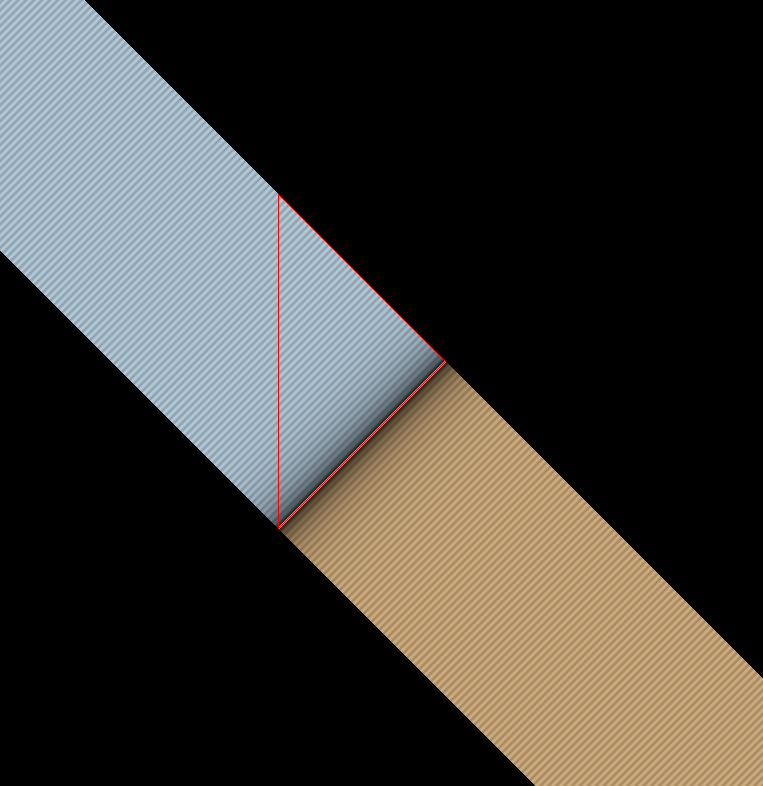
\includegraphics[width=.6\linewidth]{images/initial_segment_regions.png}
    \caption{él régiók kezdeti határai}
    \label{fig:initial_segment_regions-1}
\end{figure}

Az algoritmus következő lépéseként minden régiót elvágunk az összes többi régióhoz tartozó csúccsal és szakasszal. Eredményül a sokszög Voronoj-diagramja egy közelítését kapjuk, ahol a régiók között némi átfedés van. Ezt az átfedést a raszterizáció során a Z-puffer algoritmus oldja fel és jeleníti meg a megfelelő régiót.

\begin{figure}[H]
    \centering
    
\includegraphics[width=.6\linewidth]{images/algorithm_output_top_down.png}
    \caption{Alakzat felülnézete}
    \label{fig:algorithm_output_top_down-1}
\end{figure}
\begin{figure}[H]
    \centering
    
\includegraphics[width=.6\linewidth]{images/algorithm_output_bottom_up.png}
    \caption{Alakzat alulnézetből}
    \label{fig:algorithm_output_bottom_up-1}
\end{figure}

\subsection{Z-puffer algoritmus (Mélységi teszt)}
A mélységi teszt egy módszer a raszterizálásban arra, hogy eldöntsük, hogy az egymást átfedő geometriák közül melyik kerüljön megjelenítésre. Az algoritmus a GPU-n hajtódik végre és úgy működik, hogy rajzoláskor nem csak a képernyő színpufferébe ír, hanem egy másodlagos pufferbe (mélységi puffer), ahol számon tartja, hogy minden egyes elemhez a színpufferben milyen mélység tartozik. Az alkalmazás esetében színpufferbe csak akkor írunk, ha az új szín mélysége alacsonyabb (közelebb van a kamerához) a mélységi pufferben tárolt jelenlegi értéknél.

\subsection{Csúcs - csúcs vágások}

Azok a pontok, amelyek két pont között egyenlő távolságra helyezkednek el kollineárisak. Ebben a lépésben meghatározzuk azt az egyenest és annak a mentén végzünk egy vágást. Ez a művelet nem hagy átfedést a régióhatárok között. A \ref{fig:vertex_vertex_cut-1}-es ábrán láthatjuk a vágás eredményét.

\iffalse
Legyen \textit{a} pont a régióhoz tartozó csúcs és \textit{b} pont a sokszög egy pontja, ami segítségével a vágást szeretnénk végrehajtani \textit{V} régión. A vágás algoritmusa a következő:

\begin{algorithm}[H]
    \caption{csúcs - csúcs vágás}
    \label{alg:vertex_cut_vertex}
    \textbf{Bemenet:} A régió határait definiáló sokszög csúcspontjai \textit{V} és \textit{a}, \textit{b} csúcspontok
    \textbf{Kimenet:} A régió új határai \textit{V}'
    \begin{algorithmic}[1]
        \State $e = b - a$ \Comment{A vágás egyenesére merőleges normálvektor.}
        \If{$||e|| <= \epsilon$}
            \State \textbf{return} V \Comment{Ha a két csúcs egybeesik, akkor nem végzünk módosítást.}
        \Else
            \State $m = (a + b) * 0.5$ \Comment{Meghatározzuk a két csúcs közötti pontot.}
            \State \textbf{return} polyCut($V$, $m$, $e$) \Comment{$V$ konvex poligont elvágjuk $m$ pont és $e$ normálvektor által meghatározott egyenes mentén.}
        \EndIf
    \end{algorithmic}
\end{algorithm}
\fi

\begin{figure}[H]
    \centering
    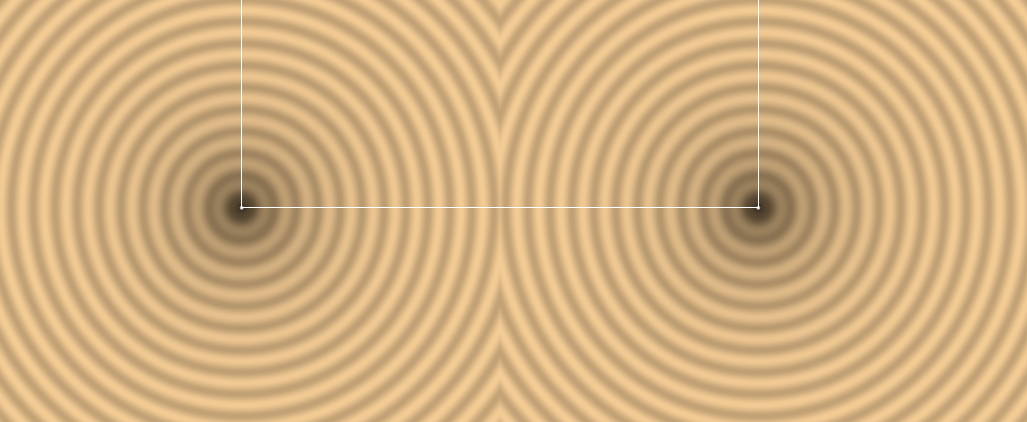
\includegraphics[width=1\linewidth]{images/vertex_vertex_cut.png}
    \caption{Csúcs - csúcs vágás eredménye}
    \label{fig:vertex_vertex_cut-1}
\end{figure}

\subsection{csúcs - él vágás} \label{vertex_segment_cut}
Azok a pontok, amelyek egy ponttól és egy egyenestől azonos távolságra vannak, egy parabolán helyezkednek el, ahol a parabola fókuszpontja megegyezik a vágási régióhoz tartozó csúccsal. Ebben a lépésben konstans számú vágást hajtunk végre a parabola görbéje mentén a csúcs régión. Minél nagyobb a vágások száma, annál pontosabb közelítést kapunk a csúcs régió Voronoj-cellájához. A \ref{fig:vertex_segment_cut-1}-as ábrán láthatjuk a vágás eredményét.

\begin{figure}[H]
    \centering
    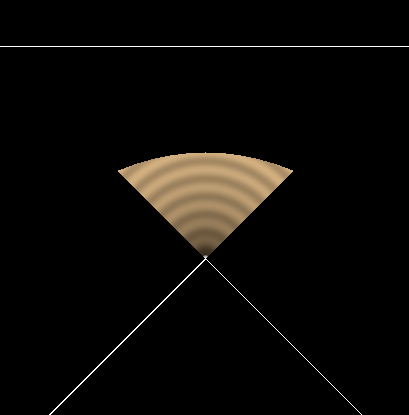
\includegraphics[width=.55\linewidth]{images/vertex_segment_cut.png}
    \caption{csúcs - él vágás eredménye}
    \label{fig:vertex_segment_cut-1}
\end{figure}

\subsection{Él - csúcs vágás}
Az él és csúcs közötti Voronoj-cella határ a csúcs oldaláról konvex, az él oldaláról egy konkáv tartományt eredményez. A \ref{vertex_segment_cut}-es szekcióban meghatároztuk a parabolát, ami a csúcshoz tartozik. A számítások leegyszerűsítése érdekében az él esetében csak egy egyenes mentén vágunk úgy, hogy a csúcs régió paraboláját lefedjük, majd raszterizáláskor a Z-puffer algoritmus segítségével kerül feloldásra az átfedés. A lépés eredménye a \ref{fig:segment_vertex_cut-1}-es ábrán látható.

\begin{figure}[H]
    \centering
    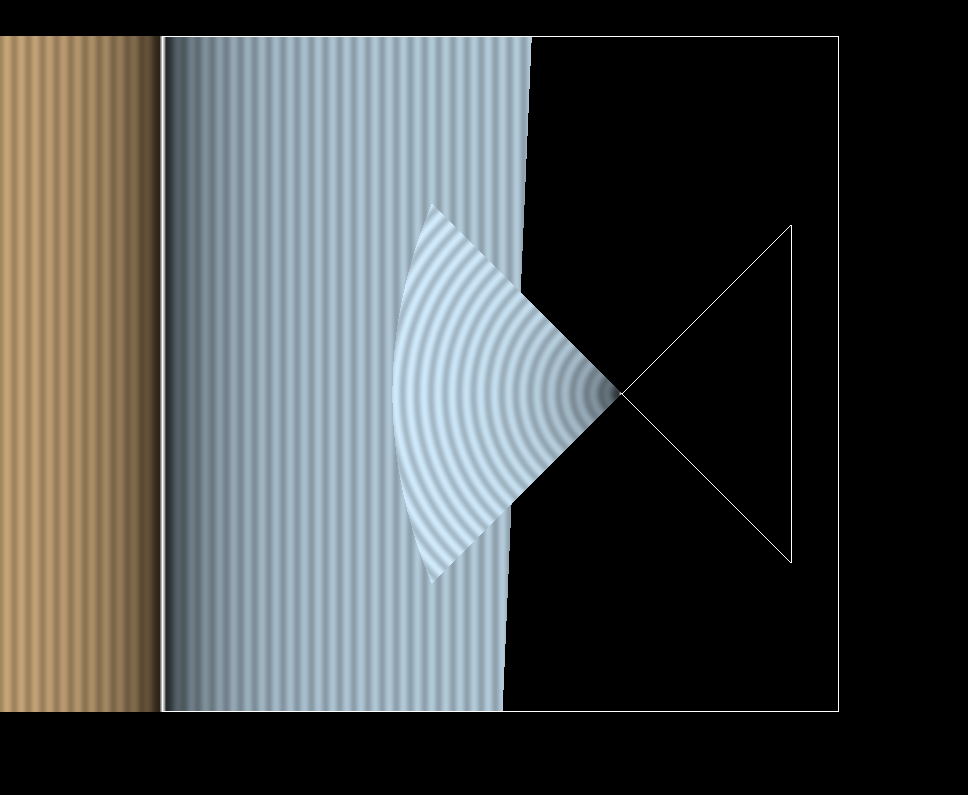
\includegraphics[width=.55\linewidth]{images/segment_vertex_cut.png}
    \caption{Él - csúcs vágás eredménye}
    \label{fig:segment_vertex_cut-1}
\end{figure}

\subsection{Él - él vágás}
Él - él vágás esetén figyelembe kell vennünk azoknak relatív pozícióját. Két él közötti rész három tartományra osztható fel: Az a tartomány, ahol az élek belső tartománya vannak közelebb egymáshoz, itt egy egyenes mentén helyezkednek el az egyenlő távolságra lévő pontok, és két olyan tartomány, ahol az egyik élhez tartozó csúcshoz vagyunk közelebb, ahol a határ parabolikus. Ebben a lépésben egyetlen egyenes mentén vágunk élenként, az egyenesből és két parabolából álló összetett görbét lefedve. A vágással átfedések keletkeznek, amit a Z-puffer algoritmus old fel. A lépés eredménye a \ref{fig:segment_segment_cut-1}-es ábrán látható.

\begin{figure}[H]
    \centering
    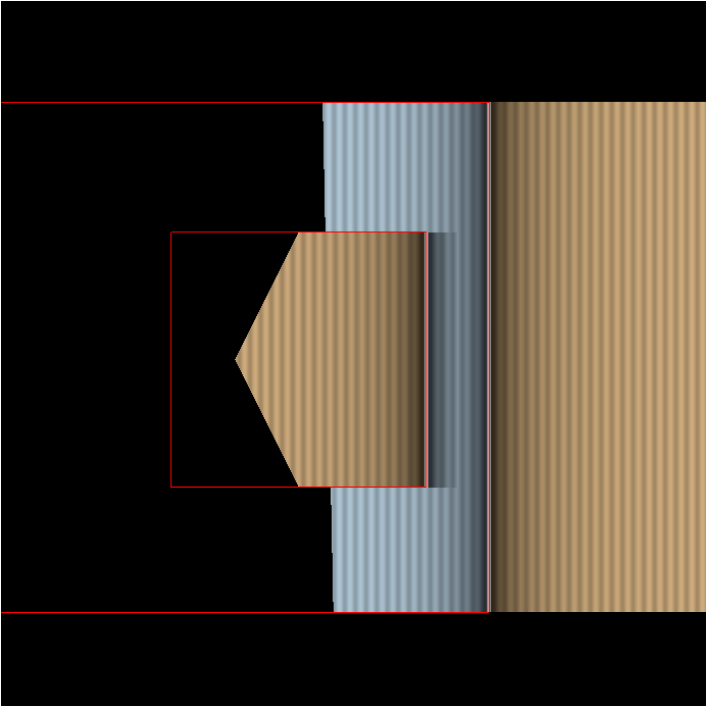
\includegraphics[width=.55\linewidth]{images/segment_segment_cut.png}
    \caption{Él - él vágás eredménye}
    \label{fig:segment_segment_cut-1}
\end{figure}

\section{A szerkesztő megtervezése}
A szerkesztő alapját az Autodesk Maya ,,construction history" funkciója inspirálta. Maya-ban a szerkesztett objektum az elvégzett műveletek sorozatából tevődik össze, ha egy köztes műveletet megváltoztatunk, akkor lehetőségünk van a rákövetkező műveleteket újra végrehajtani, közben egy teljesen eltérő eredményt kapva.

\subsection{A szerkesztő magja}

A szerkesztő tervezésében különös figyelmet kapott annak skálázhatósága bővíthetőség szempontjából, osztálydiagramját a \ref{fig:class_editor-1}-es ábrán láthatjuk. Az alakzaton parancsok kiváltásával módosíthatunk, amire válaszul a szerkesztő eseményeket vált ki, hogy az alkalmazás minden eleme értesüljön a változásról és reagálni tudjon rá. Ezen architektúra lehetővé teszi, hogy minden szerkesztőt használó modulban a szerkesztési adatok frissek legyenek még akkor is, ha számos forrásból kap bemenetet a szerkesztő.

A parancsokat felfoghatjuk állapot átmenetekként, ahol minden parancs után egy állapottal bővül a szerkesztő verme. A verem adatstruktúra természetéből adódóan a visszalépés triviális művelet, mivel csak el kell vetnünk a verem tetejéről a módosítást. Az alkalmazásban a teljesítményre való tekintettel a veremben az átmenet által készített új állapot is tárolásra kerül, így minimalizálva a potenciálisan nagy számításigényű műveletek túlzott számban való kiértékelését. \textit{Megjegyzés: A jelenlegi implementáció nem támogatja az előrelépés és a köztes műveletek módosítását.}

\begin{figure}[H]
    \centering
    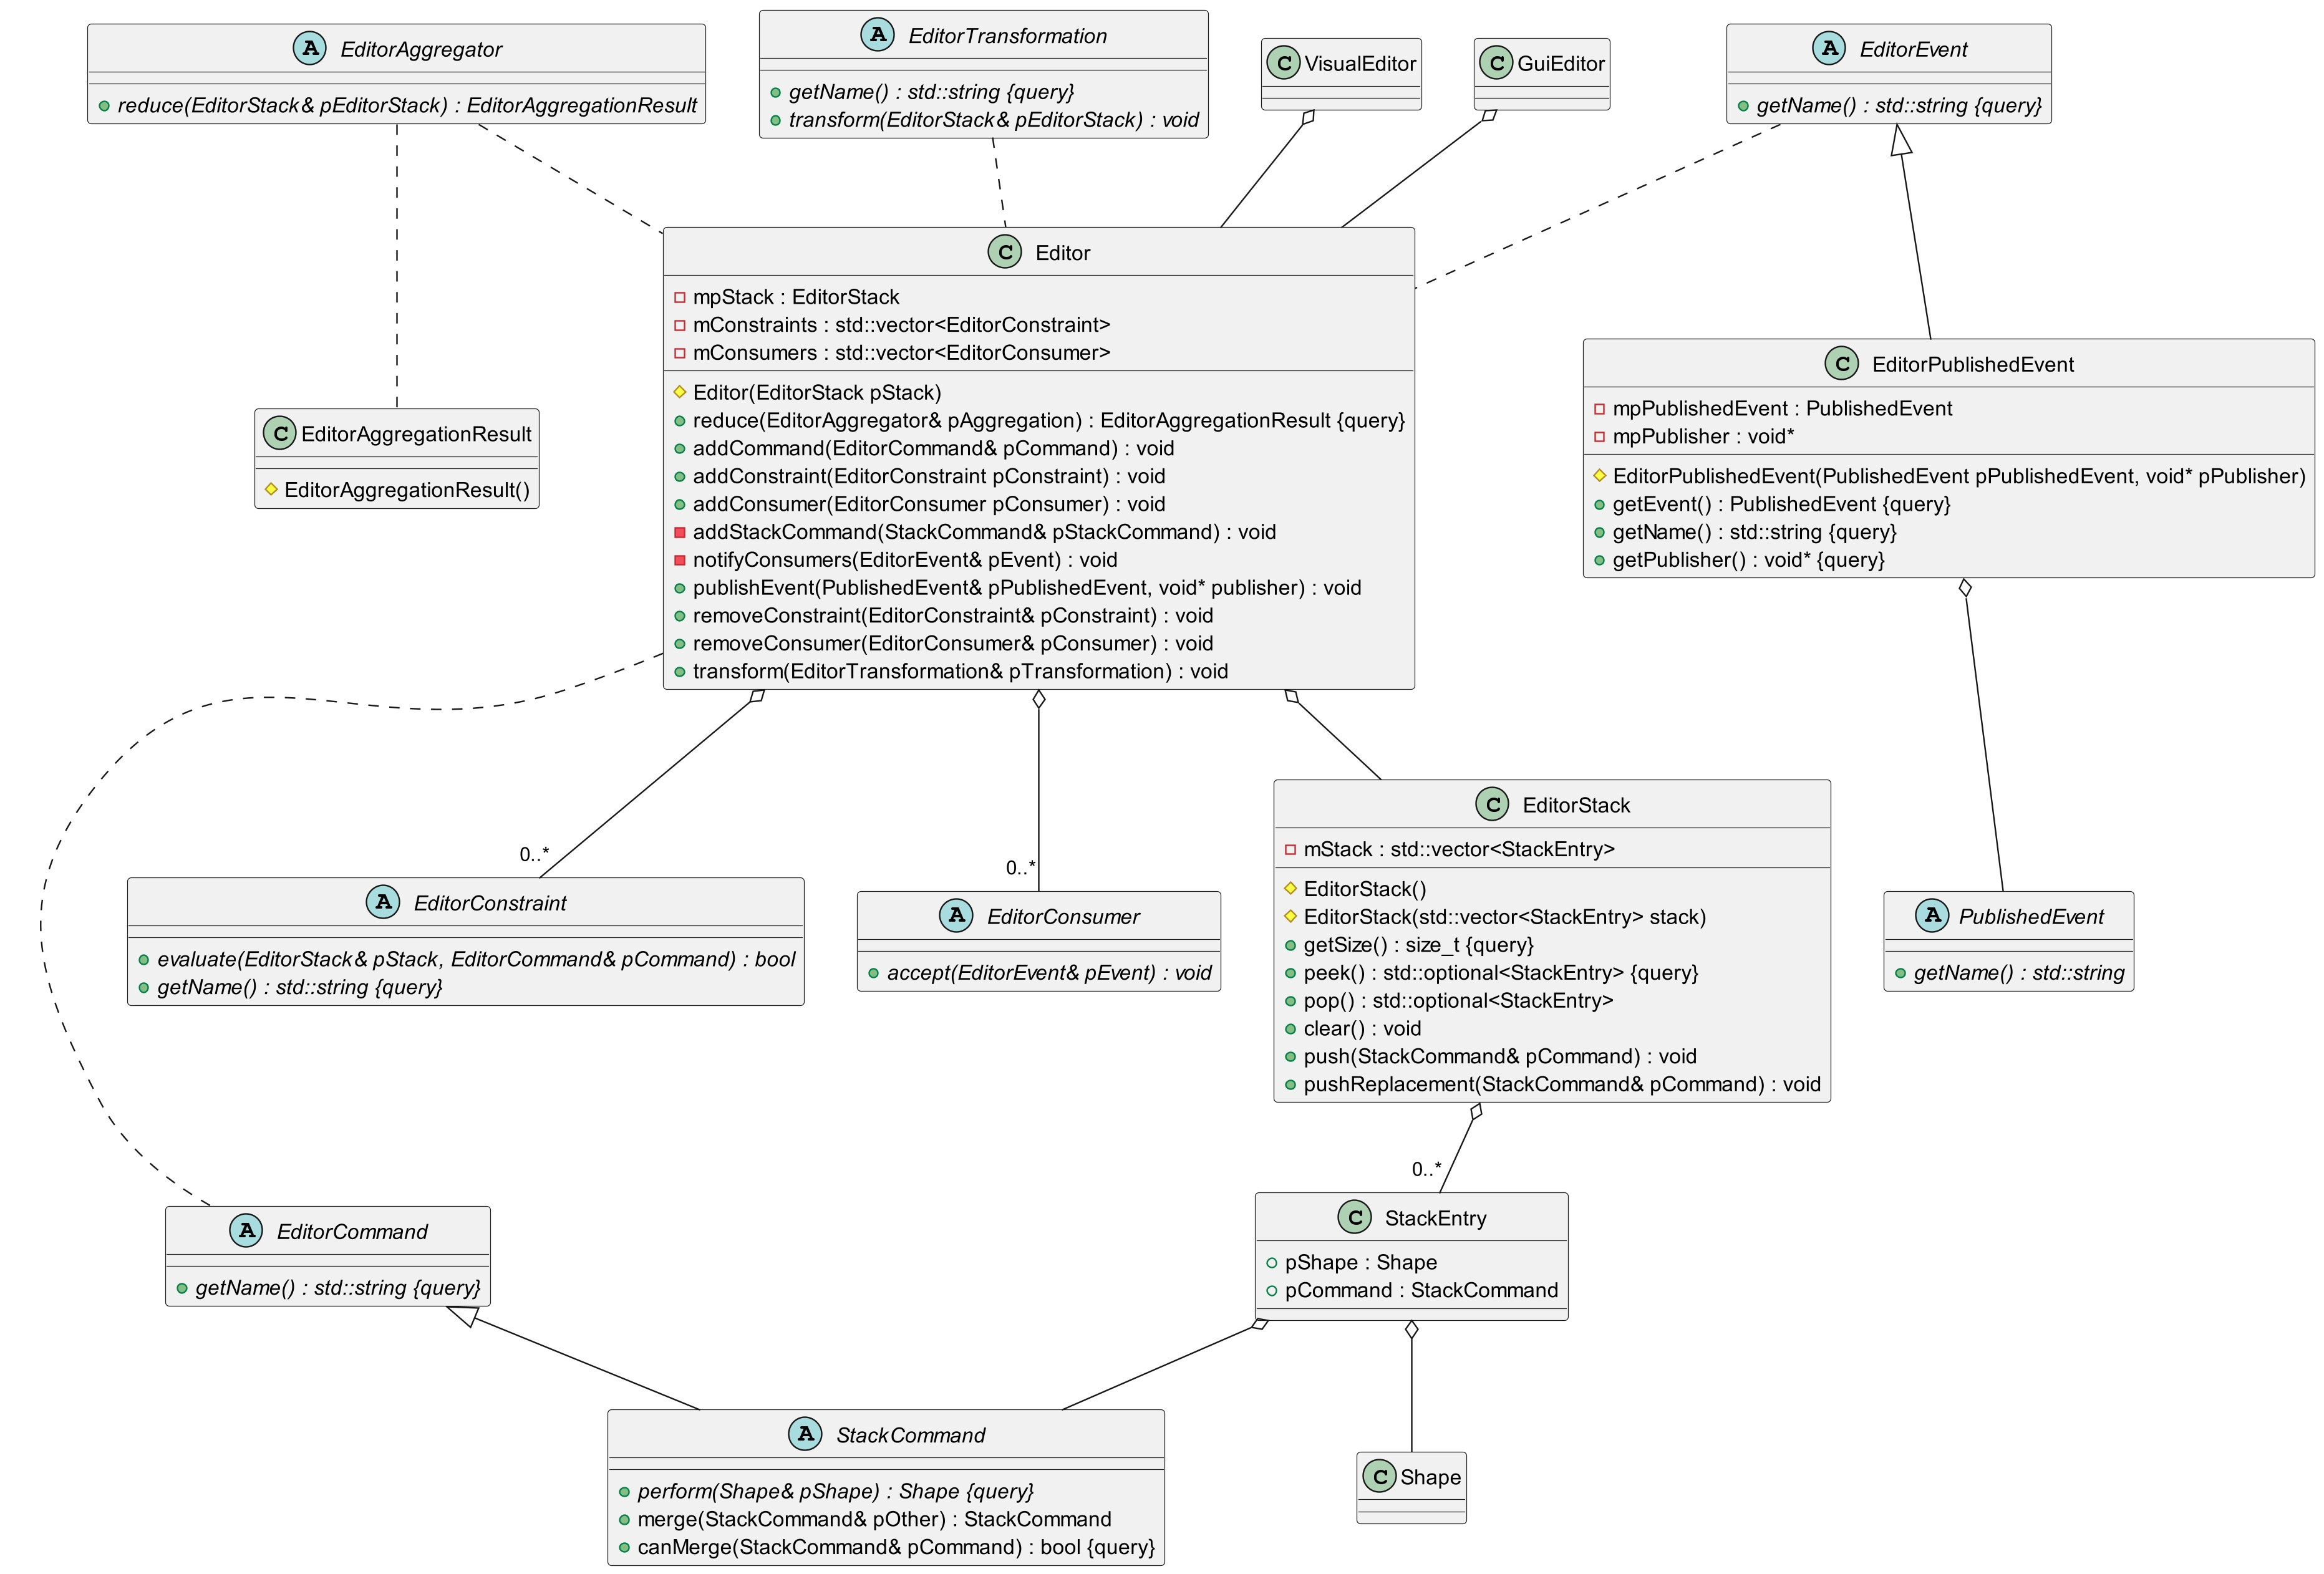
\includegraphics[width=1\linewidth]{images/class_editor.png}
    \caption{Szerkesztő osztálydiagramja}
    \label{fig:class_editor-1}
\end{figure}


\subsection{Szerkesztői parancsok}

A szerkesztői parancs (\textbf{EditorCommand}) egy általános típus, egyetlen művelete annak nevének lekérése a szándék ezzel az interfésszel, hogy a szerkesztő eltérő hatáskörű parancsokat is le tudjon kezelni.

A verem parancs (\textbf{StackCommand}) ennek egy olyan specializációja, ami egy alakzatból egy új alakzatot készít a \textit{perform} metódus segítségével. A definiált műveletnek szigorúan tisztának kell lennie. Az osztálydiagram az implementációkkal a \ref{fig:class_editor_command-1}-es ábrán láthatóak.

A verem parancsok egyesíthetőek, amennyiben az eredmény értelmezhető. Akkor hajthatjuk végre az egyesítést, ha a \textit{canMerge} metódus igazat ad vissza a parancsra, amivel meghívjuk, ekkor a \textit{merge} metódus végzi el az egyesítést. Az egyesítés rendelkezik alap implementációval, ami letiltja ezt a viselkedést. Erre a műveletre azért volt szükség, mert a vizuális szerkesztő esetében ugyanazt a csúcsot vagy poligont pár másodperc alatt akár ezerszer is elmozdíthatjuk, ami egyesítés nélkül 1000 új bejegyzést hozna létre a szerkesztői veremben.

\begin{figure}[H]
    \centering
    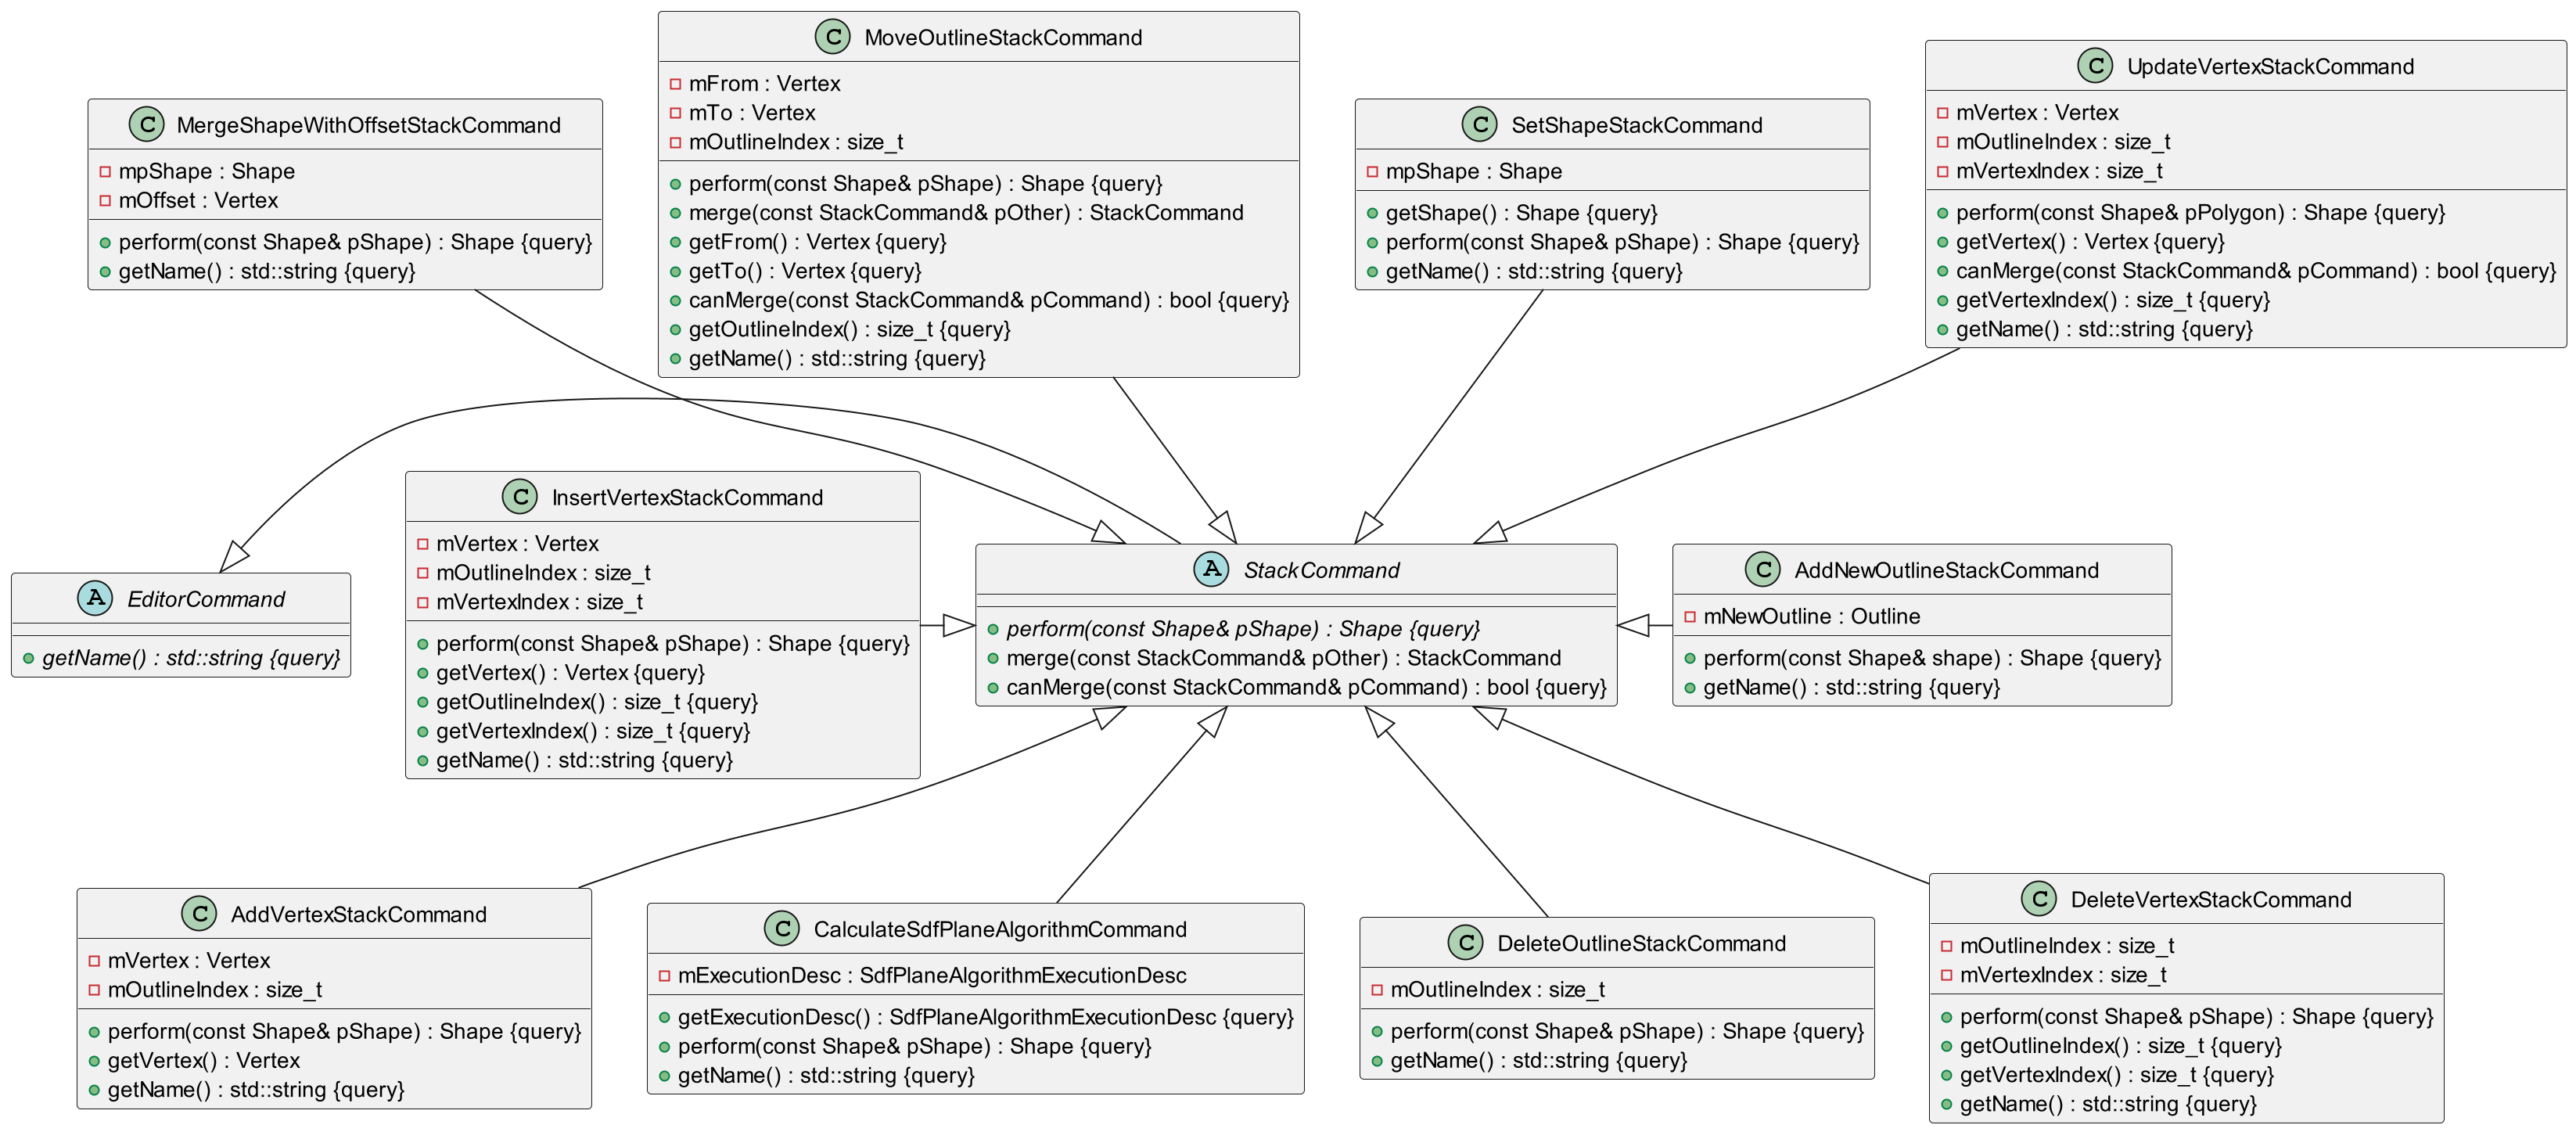
\includegraphics[width=1\linewidth]{images/class_editor_command.png}
    \caption{A szerkesztőben rendelkezésre álló parancsok osztálydiagramja}
    \label{fig:class_editor_command-1}
\end{figure}

\textbf{A StackCommand osztály implementációi}

\begin{description}
    \item[AddNewOutlineStackCommand] Hozzáadja az alakzathoz a megadott poligont.
    \item[AddVertexStackCommand] Az egyik poligonhoz hozzáad egy csúcsot a lista végére.
    \item[CalculateSdfPlaneAlgorithmCommand] Végrehajtja az algoritmust az alakzaton.
    \item[DeleteOutlineStackCommand] Töröl egy poligont az alakzatból.
    \item[DeleteVertexStackCommand] Töröl egy csúcsot az egyik poligonból.
    \item[InsertVertexStackCommand] Az egyik poligonhoz hozzáad egy csúcsot a lista egy megadott indexére.
    \item[MergeShapeWithOffsetStackCommand] A megadott alakzatot egyesíti a szerkesztőével.
    \item[MoveOutlineStackCommand] Elmozdít egy poligont az alakzatban két referencia pont segítségével. Ez a művelet egyesíthető egy azonos típusú paranccsal, ha ugyanazt a poligont mozgatják, ugyanabból a kiindulópontból.
    \item[SetShapeStackCommand] Lecseréli az alakzatot.
    \item[UpdateVertexStackCommand] Frissíti egy csúcs értékét az egyik poligonban. Ez a művelet egyesíthető egy azonos típusú paranccsal, ha pontosan ugyanazt a csúcsot mozgatják.
\end{description}

\subsection{Szerkesztő összesítő műveletek}

Az alkalmazásban szükség van olyan műveletre, amik a szerkesztő vermének állapotát összesítik, például a tárolt műveletek számát megadják. Erre a célra lett létrehozva a \textbf{EditorAggregator} osztály, két absztrakt metódussal rendelkezik, egyik a művelet megnevezésére, a másik az összesítés végrehajtására és az eredmény visszaadására, ami a szerkesztő állapotán nem módosíthat. Minden összesítő osztály \textbf{EditorAggregationResult} típusú eredményt adhat vissza. A művelet osztálydiagramja a \ref{fig:class_editor_aggregator-1}-as ábrán látható.

\begin{figure}[H]
    \centering
    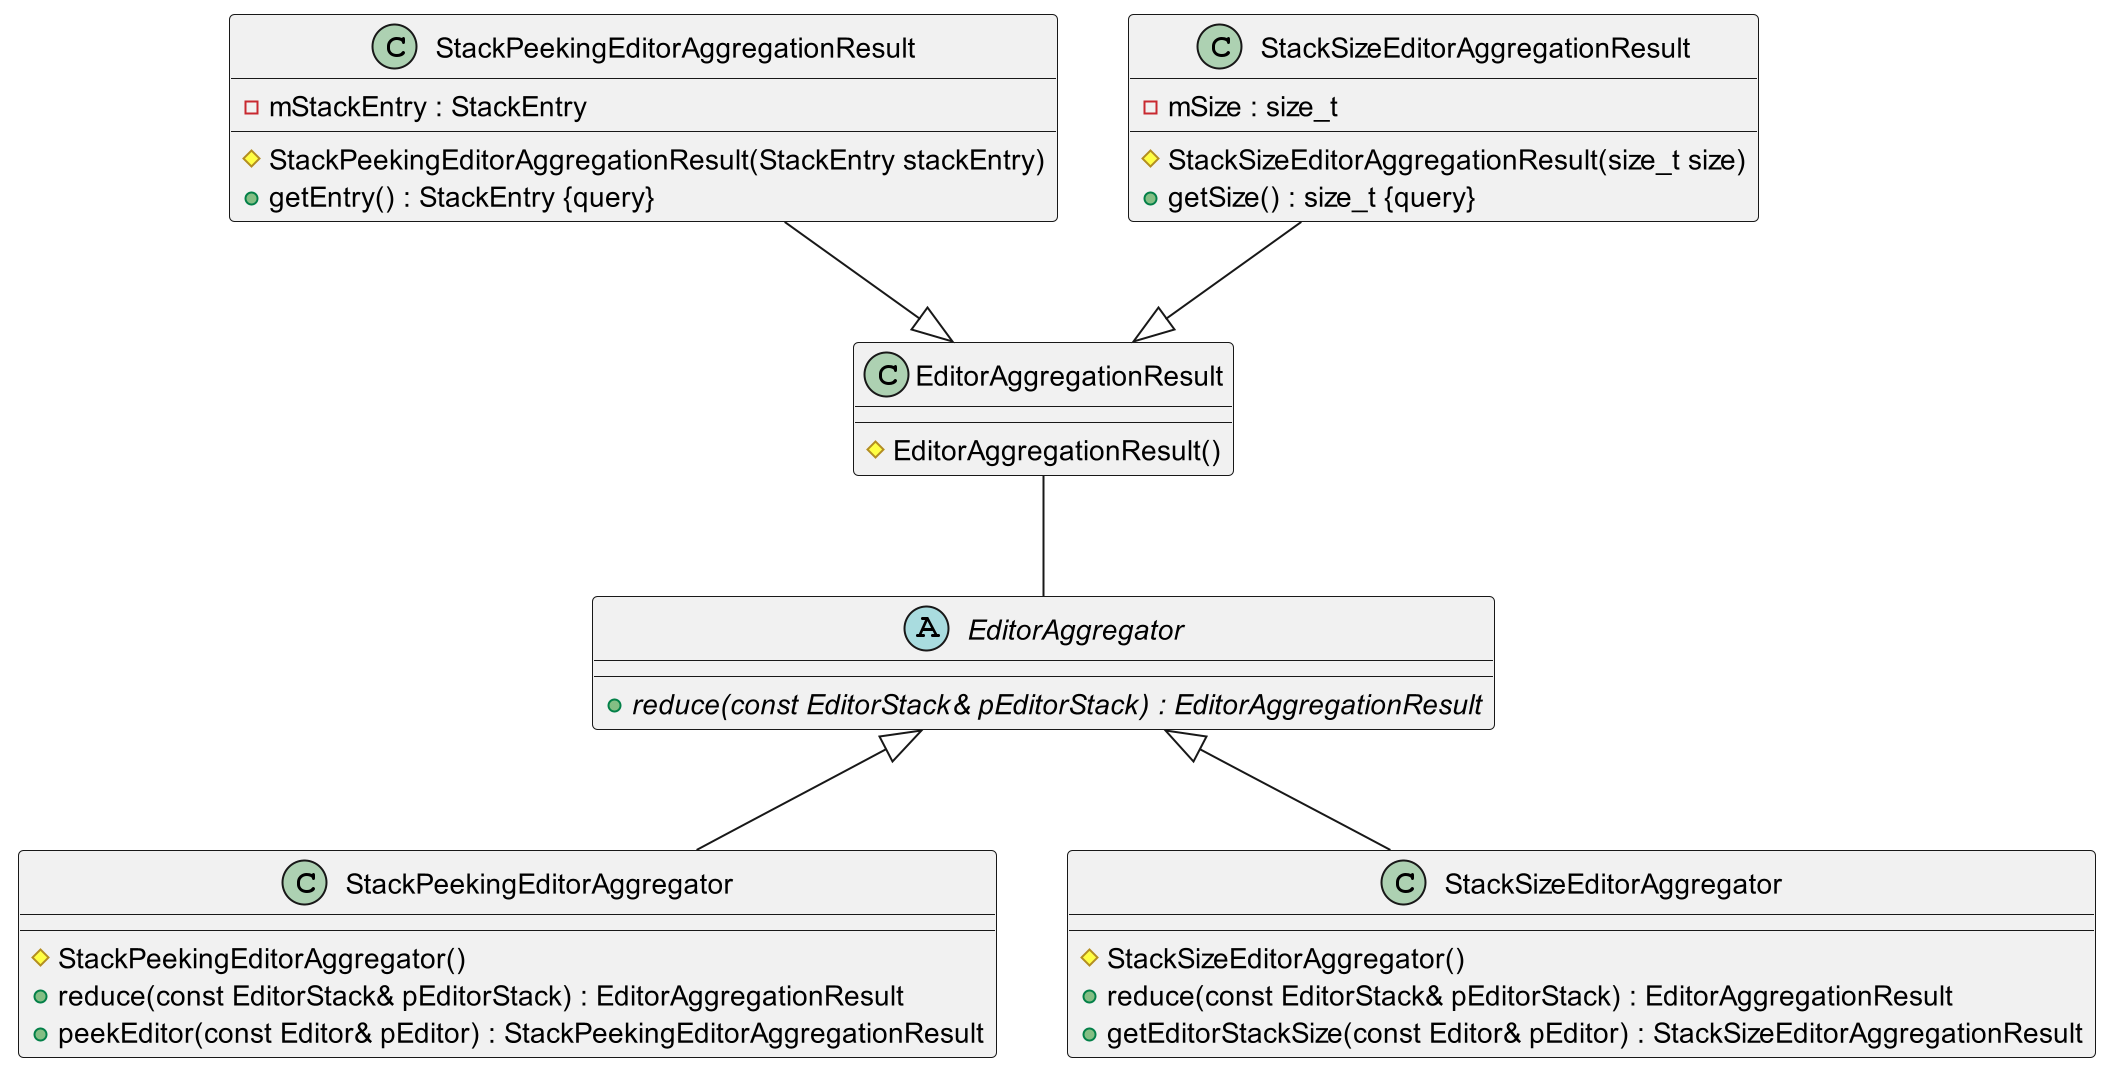
\includegraphics[width=1\linewidth]{images/class_editor_aggregator.png}
    \caption{A szerkesztői összesítések osztálydiagramja}
    \label{fig:class_editor_aggregator-1}
\end{figure}

\textbf{Az osztály implementációi}

\begin{description}
    \item[StackPeekingEditorAggregator] Visszaadja a legfelső bejegyzést a szerkesztő verméből.
    \item[StackSizeEditorAggregator] Visszaadja a verem méretét.
\end{description}

\subsection{Szerkesztői megszorítások}

Bizonyos esetekben egy változtatást nincs értelme végrehajtani egy alakzaton, például egy háromszögből nem törölhetünk csúcsot, mert akkor már nem egy sokszögről beszélünk. Az \textbf{EditorConstraint} osztályban kettő absztrakt metódus található, egyik a megszorítás azonosítására (\textit{getName}), a másik egy parancsra és a jelenlegi alakzatra megmondja, hogy a parancsban végrehajtandó művelet elvégezhető-e (\textit{evaluate}).

\begin{figure}[H]
    \centering
    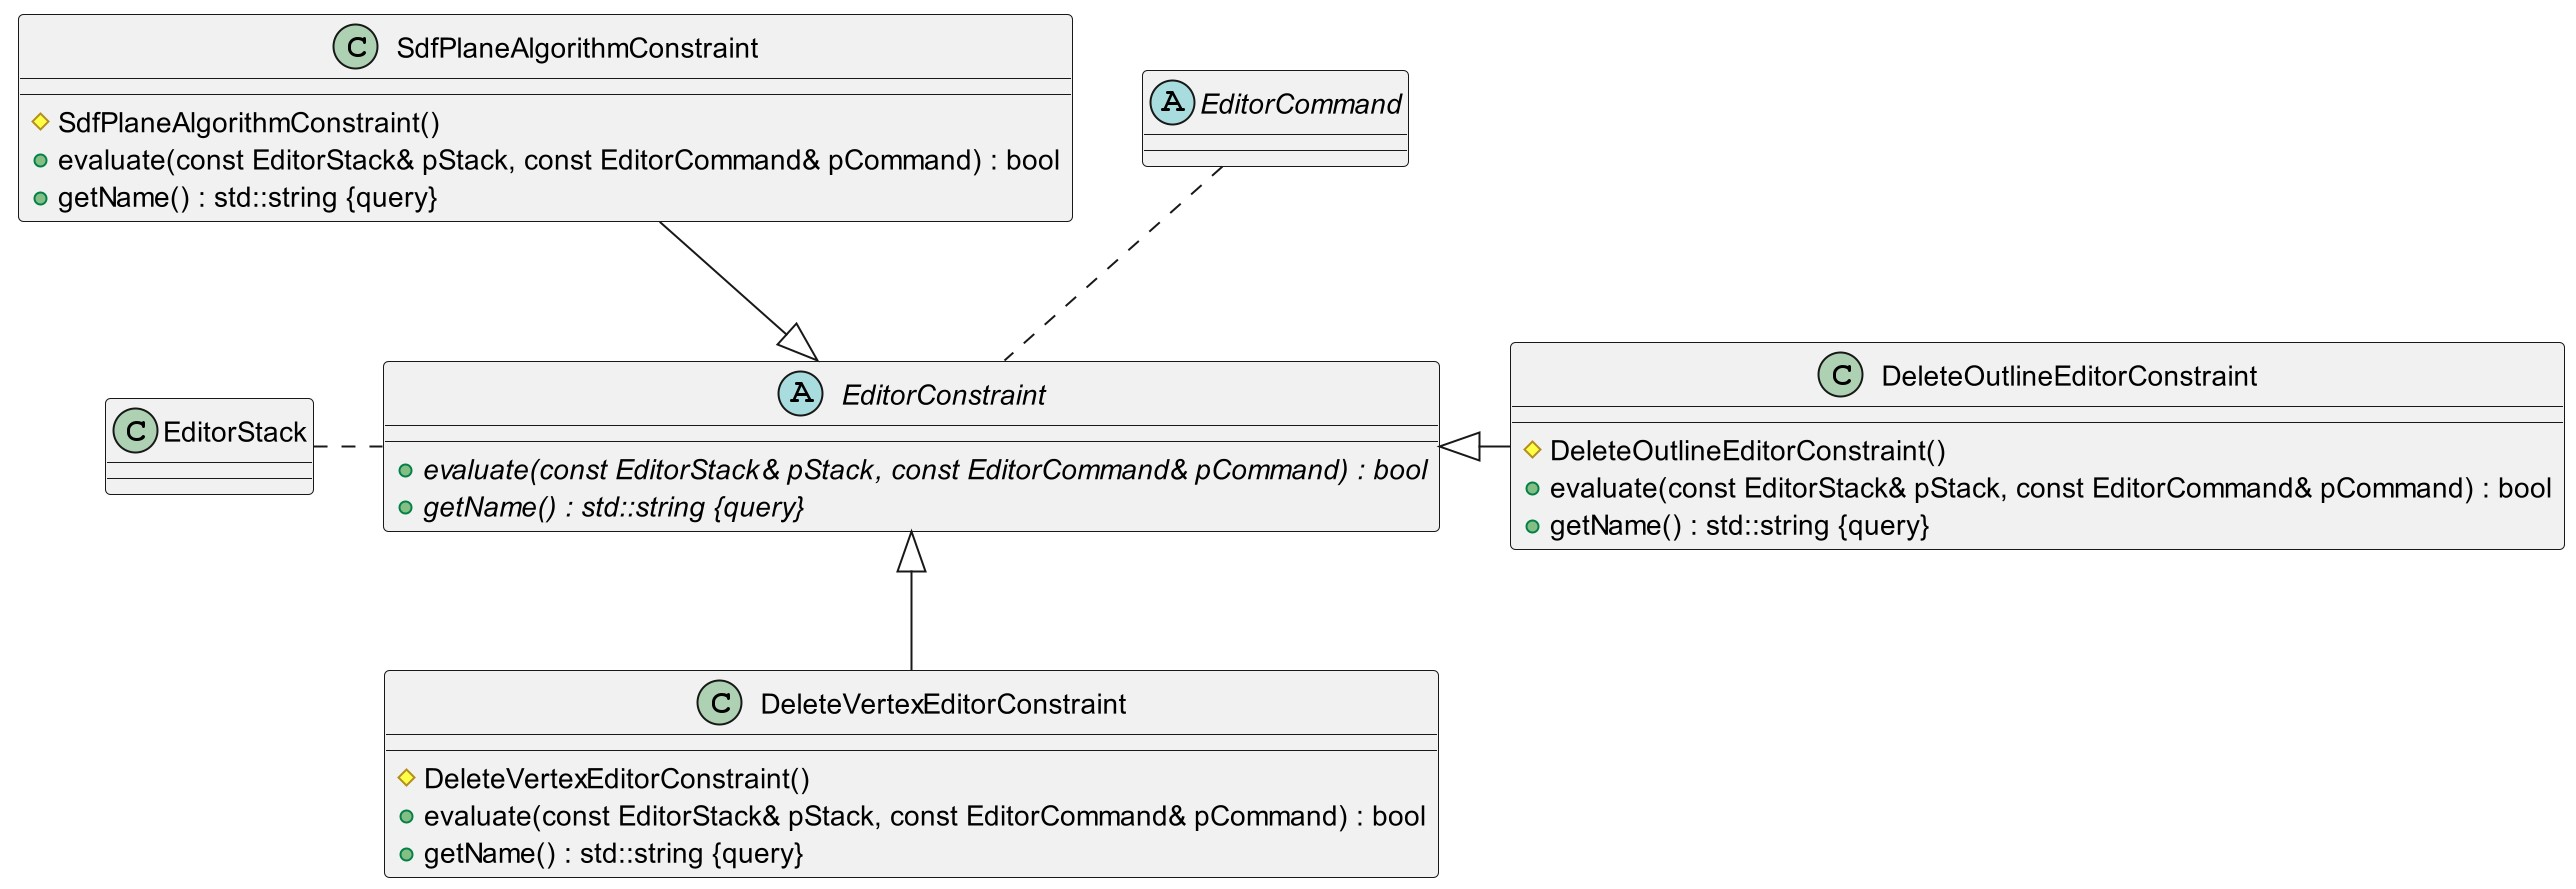
\includegraphics[width=1\linewidth]{images/class_editor_constraint.png}
    \caption{A szerkesztői megszorítások osztálydiagramja}
    \label{fig:class_editor_constraint-1}
\end{figure}

\textbf{Az osztály implementációi}

\begin{description}
    \item[DeleteOutlineEditorConstraint] Tiltja a \textbf{DeleteOutlineStackCommand} példányú parancsokat, amennyiben nem maradna az alakzatban poligon a törlés után.
    \item[DeleteVertexEditorConstraint] Tiltja a \textbf{DeleteVertexStackCommand} típusú parancsokat, amennyiben a kiválasztott poligonban kevesebb mint három pont maradna törlés után.
    \item[SdfPlaneAlgorithmConstraint] Az algoritmus nem értelmezett önmetsző alakzatokra. Ez a megszorítás tiltja a \textbf{CalculateSdfPlaneAlgorithmCommand} típusú parancsokat, ha az alakzatban vannak egymást metsző élek. Szomszédos éleket nem vesz figyelembe.
\end{description}

\subsection{Szerkesztői transzformációk}

Az eddig felsorolt osztályoknak többek között egy dologban egyeztek meg, nem módosították közvetlenül a szerkesztő állapotát.

Az \textbf{EditorTransformation} interfész kettő absztrakt metódussal rendelkezik, egyik az osztály azonosítására (\textit{getName}), a másik a verem módosításához (\textit{transform}).

\begin{figure}[H]
    \centering
    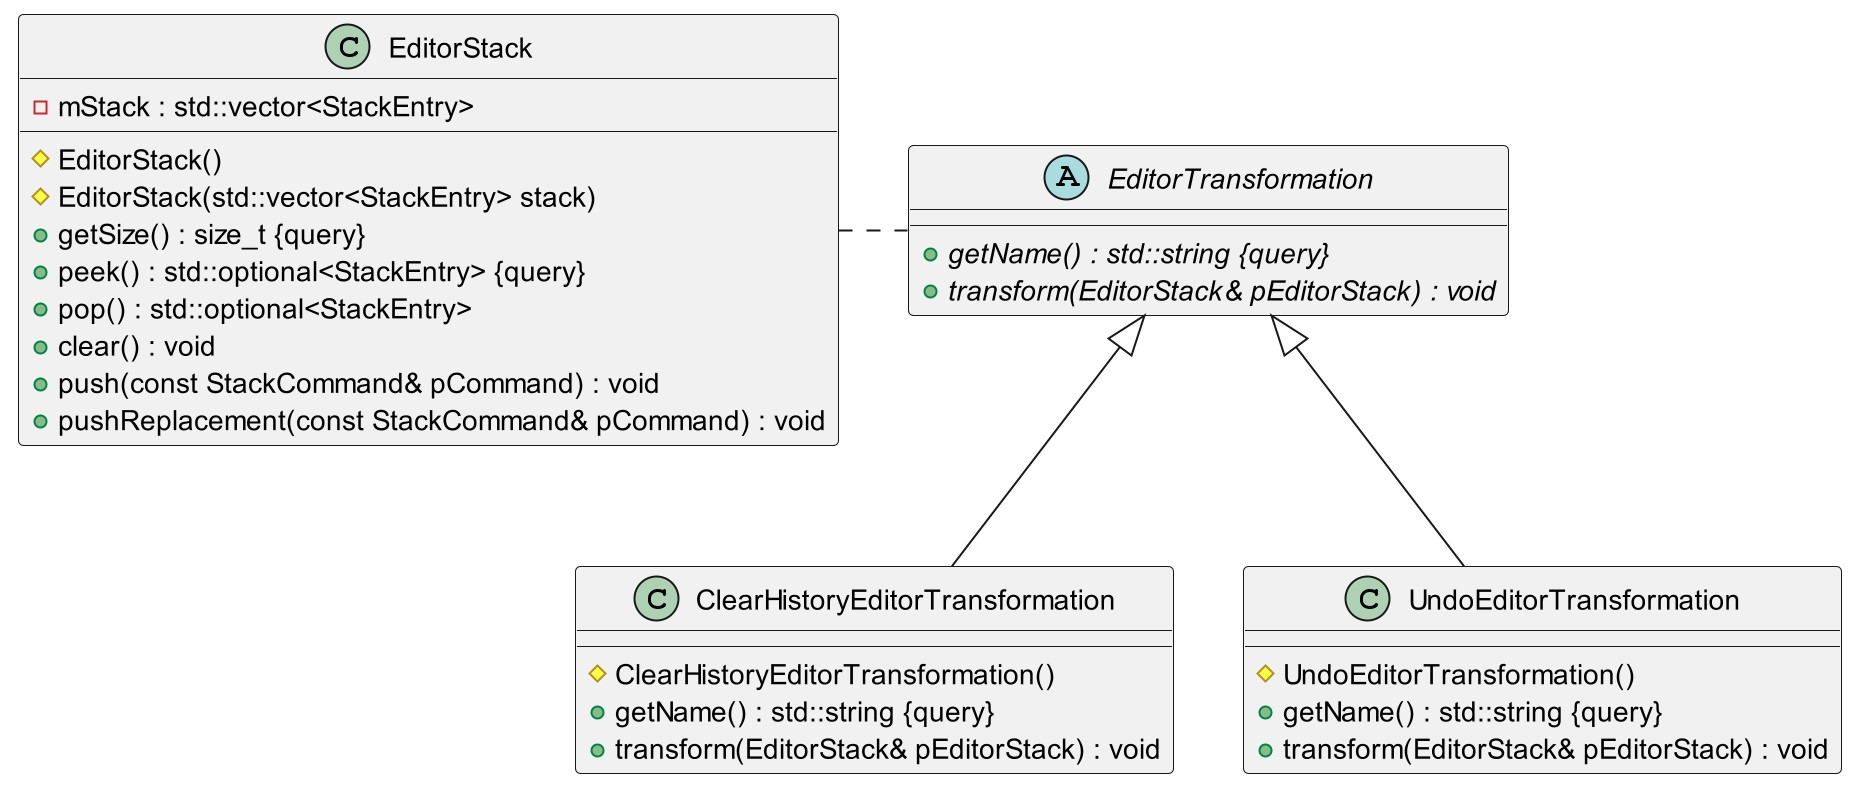
\includegraphics[width=1\linewidth]{images/class_editor_transformation.png}
    \caption{A szerkesztői transzformációk osztálydiagramja}
    \label{fig:class_editor_transformation-1}
\end{figure}

\textbf{Az osztály implementációi}

\begin{description}
    \item[ClearHistoryEditorTransformation] A szerkesztés során számos állapotváltozás bekövetkezhet az alakzatunkon. A felhasználónak a feladata a köztes állapotokat kitörölni, amikor úgy dönt, hogy azokra már biztos nincs szükség. Ez az osztály csak a legújabb állapotot hagyja meg a veremben, minden mást töröl.
    \item[UndoEditorTransformation] Lehetővé teszi a visszalépést az alakzat előző állapotára. Ezt úgy teszi, hogy a verem legújabb állapotát törli. A törlést csak akkor hajtja végre, ha a törlés után marad bejegyzés a veremben.
\end{description}


\subsection{Szerkesztői események}

A szerkesztő \textbf{EditorEvent} típusú objektumokkal értesíti az alkalmazás komponenseit, amikor valamilyen bemenetet kap, így gondoskodva arról, hogy a legfrissebb állapot szerepeljen mindenhol. Az osztályban egyetlen absztrakt metódus szerepel: (\textit{getName}), ami segítségével azonosíthatjuk az eseményt.

\begin{figure}[H]
    \centering
    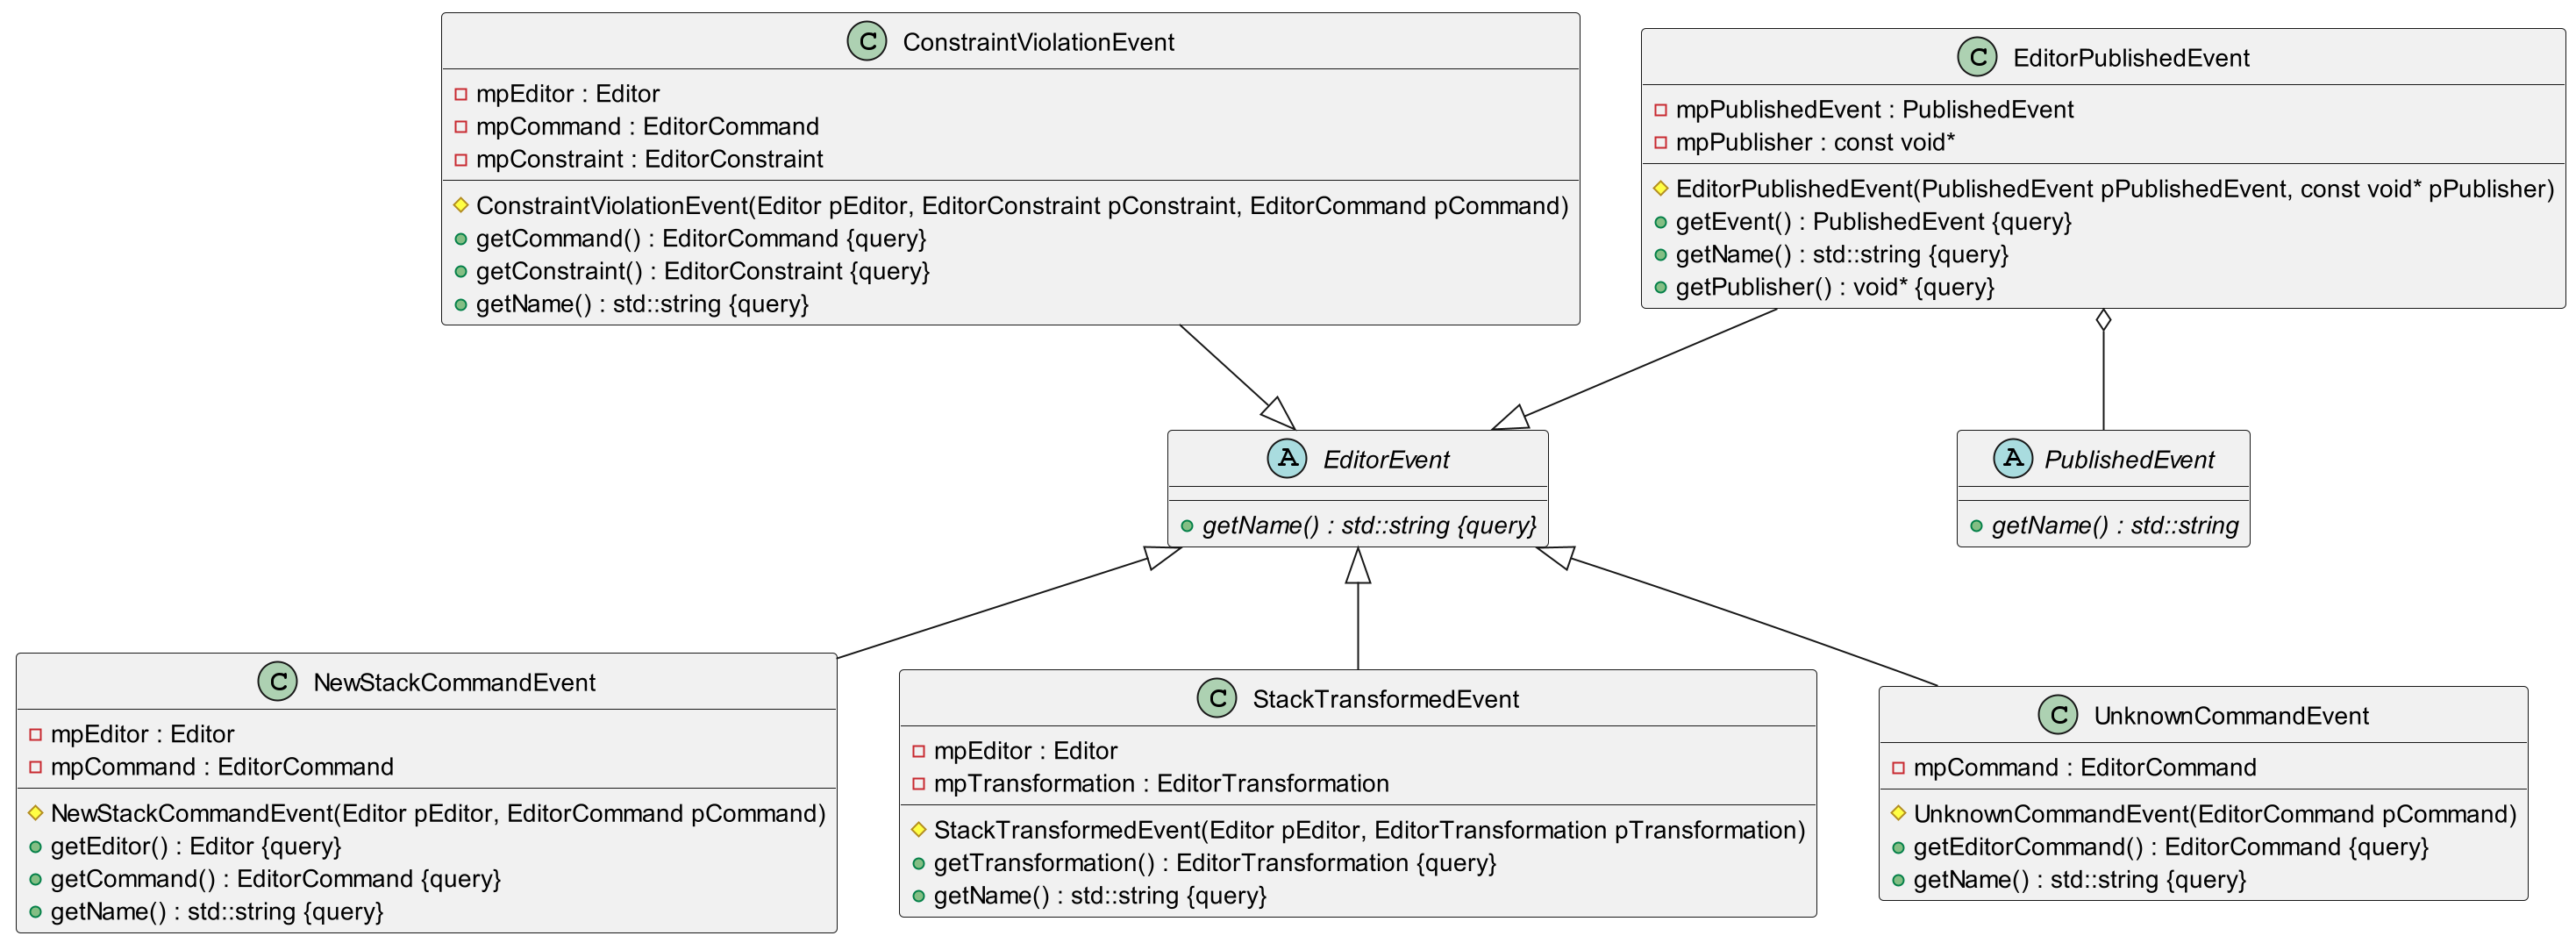
\includegraphics[width=1\linewidth]{images/class_editor_event.png}
    \caption{A szerkesztői események osztálydiagramja}
    \label{fig:class_editor_event-1}
\end{figure}

\textbf{Az osztály implementációi}

\begin{description}
    \item[NewStackCommandEvent] A szerkesztőben történt sikeres állapotátmenetek következtében kerül kiváltásra, az implementáció tartalmaz egy referenciát a kiváltott parancsra.
    \item[StackTransformedEvent] A szerkesztői transzformációk hatására váltódik ki, tárolják a módosítást végző objektumot.
    \item[ConstraintViolationEvent] Kiváltásra kerül, amennyiben egy átmenet nem hajtható végre, mert egy megszorítás sérül. A komponensek ezen az eseményen keresztül értesülnek arról, hogy pontosan mi akadályozta meg az új állapot létrehozását.
    \item[UnknownCommandEvent] Kiváltódik, ha a szerkesztő nem tudja feldolgozni a beadott \textbf{EditorCommand} implementációt. Jelenleg minden osztályra hibát ad a szerkesztő, ami nem a \textbf{StackCommand} leszármazottja.
    \item[EditorPublishedEvent] Egyedi események beküldésekor kerül kiváltásra ez az esemény, tárol egy egyedi azonosítót a küldőről, ami általában a küldő objektum memóriacíme és egy \textbf{PublishedEvent} típusú objektumot, ami a közzétételre szánt információt tartalmazza.
\end{description}

\subsection{Kommunikáció komponensek között}

Az alkalmazás komponensei szabadon kommunikálhatnak egymással a Publikáló-feliratkozó minta segítségével a szerkesztőn keresztül. Az üzenetküldés úgy történik, hogy meghívjuk a \textit{publishEvent} metódusát a szerkesztőnek a \textbf{PublishedEvent} típusú objektumunkkal, amit üzenetként szeretnék küldeni. Erre a szerkesztő kivált egy \textbf{EditorPublishedEvent} típusú eseményt, amivel kézbesíti minden feliratkozott komponensnek.

\begin{figure}[H]
    \centering
    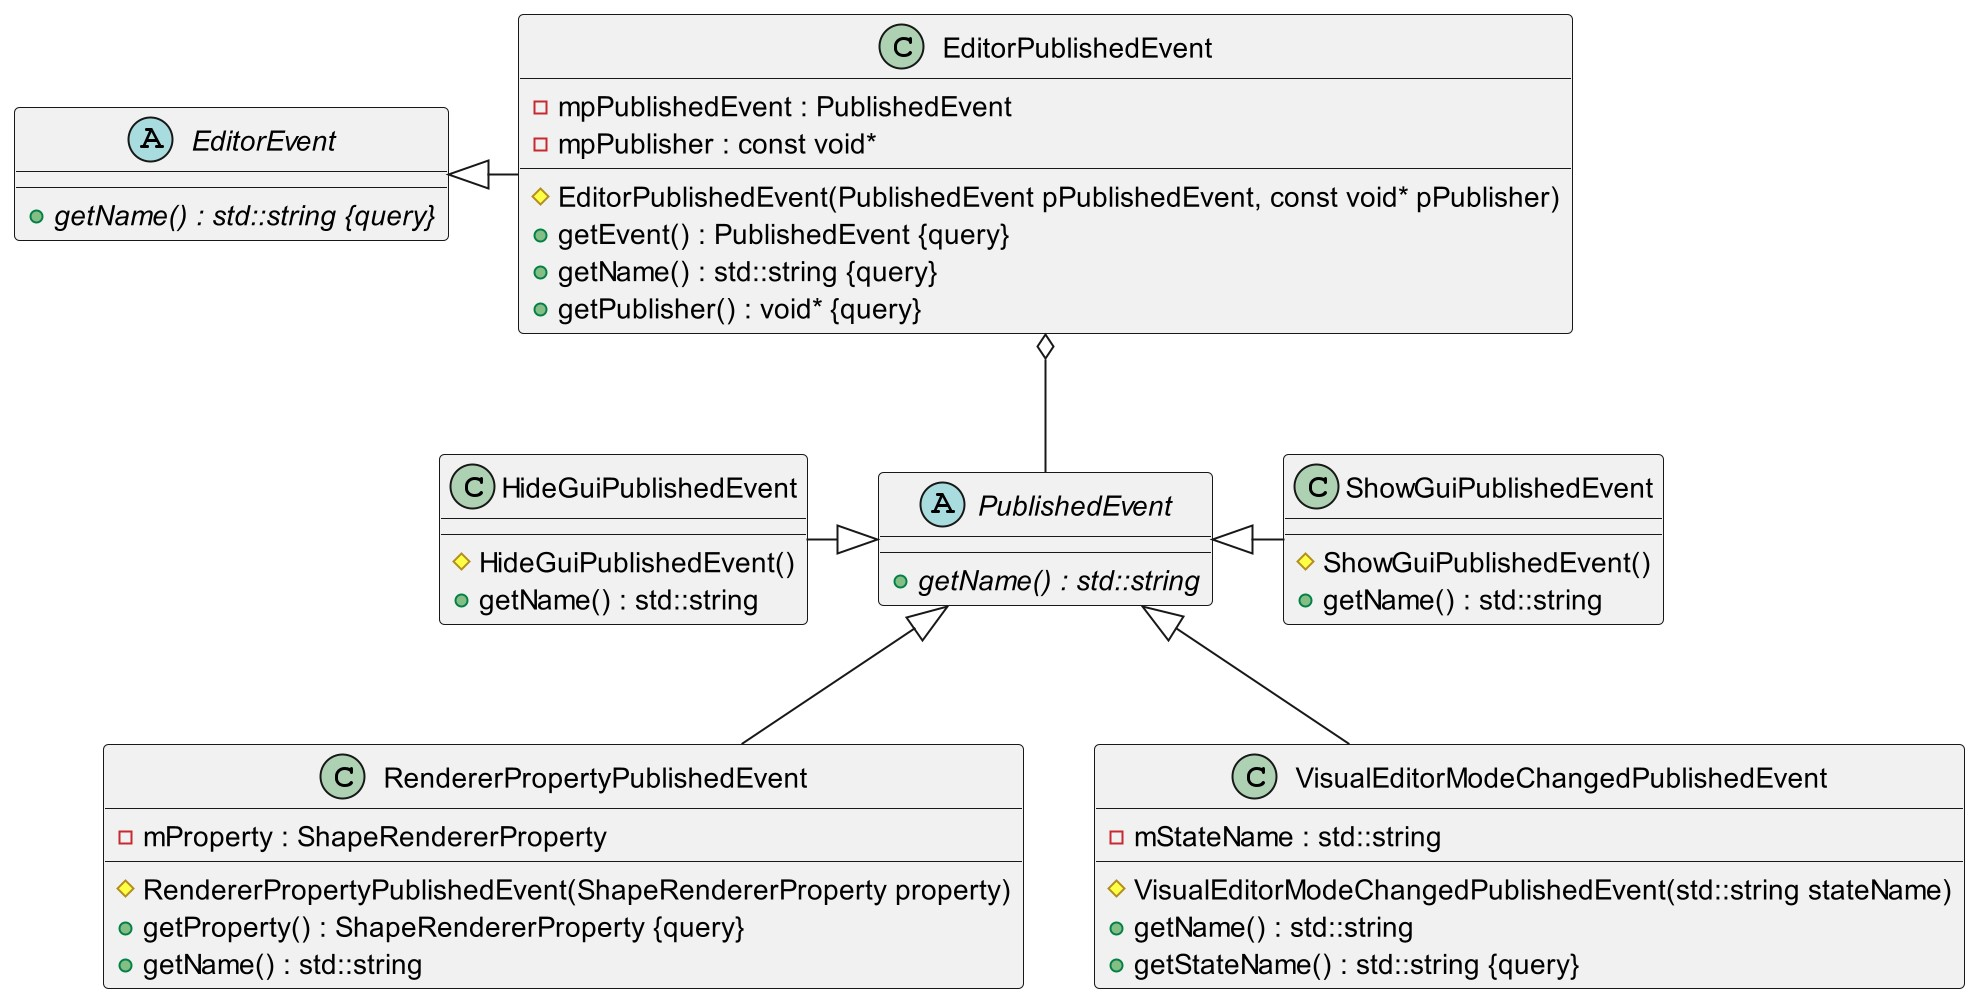
\includegraphics[width=1\linewidth]{images/class_editor_published_event.png}
    \caption{Az üzenetküldésre használt osztályok diagramja}
    \label{fig:class_editor_published_event-1}
\end{figure}

\textbf{Az osztály implementációi}

\begin{description}
    \item[HideGuiPublishedEvent] Parancs a GUI szerkesztőnek, hogy ne jelenítse meg a felhasználói felületet. A 3D nézet aktiválásakor váltódik ki. A GUI láthatósága nem változik a következő parancsig.
    \item[ShowGuiPublishedEvent] Parancs a GUI szerkesztőnek, hogy jelenítse meg a felhasználói felületet.
    \item[RendererPropertyPublishedEvent] A megjelenítés stílusának változtatásához használt esemény, a beállítás kulcsát és egy új értéket tartalmaz.
    \item[VisualEditorModeChangedPublishedEvent] A vizuális szerkesztő ezzel hírdeti ki, hogy épp milyen eszköz van kiválasztva, az aktív eszköz megjelenítéséhez a GUI-n van használva.
\end{description}

\subsection{Szerkesztői események feldolgozása}

Az alkalmazásban \textbf{EditorConsumer} típusú objektumokat iratkoztathatunk fel és le a szerkesztőben az események fogadására. Az osztályban egy absztrakt metódus van (\textit{accept}) az események fogadására.

\begin{figure}[H]
    \centering
    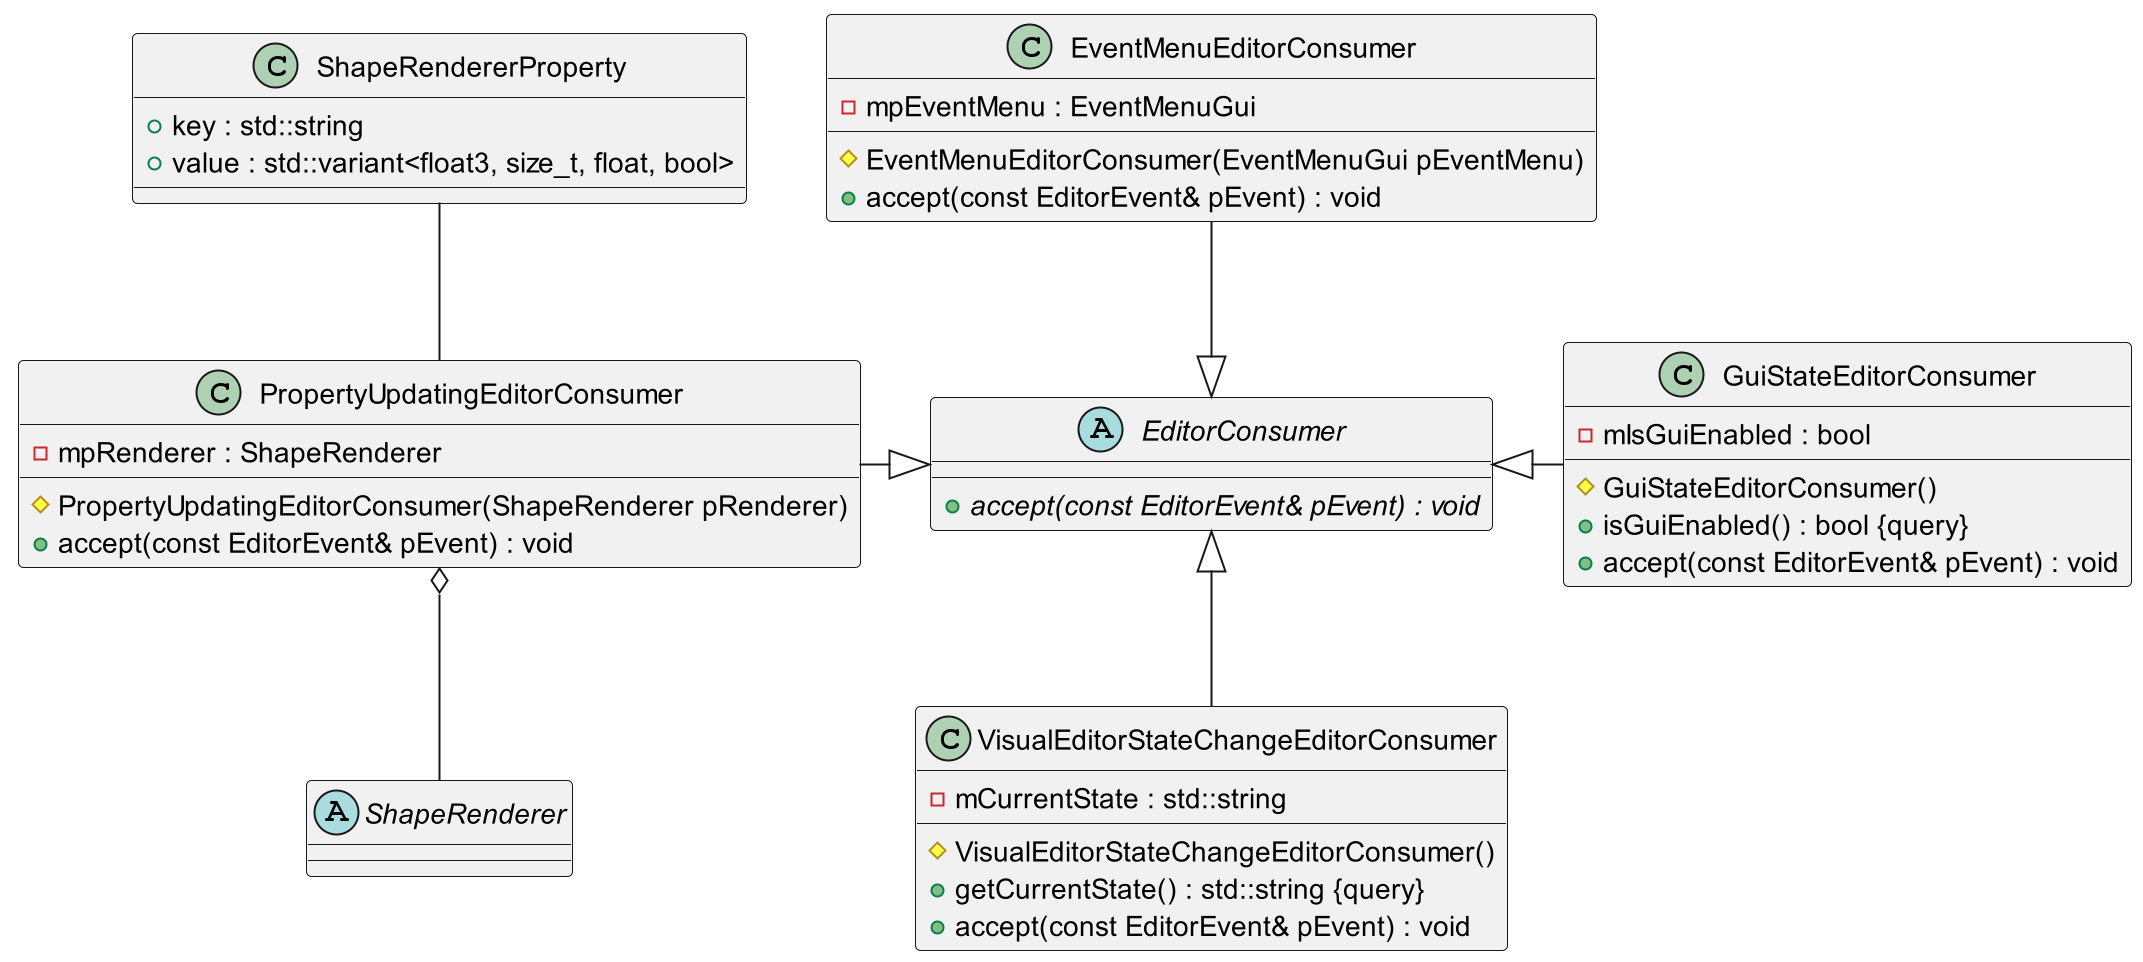
\includegraphics[width=1\linewidth]{images/class_editor_consumer.png}
    \caption{Az eseményfeldolgozó osztálydiagramja}
    \label{fig:class_editor_consumer-1}
\end{figure}

\textbf{Az osztály implementációi}

\begin{description}
    \item[EventMenuEditorConsumer] Minden beérkező eseményt lement egy listában, ami később az eseménymenün kerül megjelenítésre.
    \item[GuiStateEditorConsumer] Figyel a \textbf{HideGuiPublishedEvent} és \textbf{ShowGuiPublishedEvent} üzenetekre és számon tartja, hogy egy pillanatban meg kell-e jeleníteni a GUI-t.
    \item[PropertyUpdatingEditorConsumer] Feldolgozza a \textbf{RendererPropertyPublishedEvent} típusú objektumokat, frissíti az adattagként tárolt \textbf{ShapeRenderer} kulcsát a kapott értékkel.
    \item[VisualEditorStateChangedEditorConsumer] Feldolgozza a \textbf{VisualEditorModeChangedPublishedEvent} típusú eseményeket vizuális szerkesztő aktív eszközének számontartásához.
\end{description}


\section{GUI szerkesztő}

Az alkalmazás felhasználói felülete szöveg, gombok és beviteli mezők csoportjaiból áll szerepkör szerint. Ami közös bennünk, hogy mindegyik adatforrása a szerkesztő magja, amihez példányosításkor referenciát kapnak, majd a referencián keresztül iratkoznak fel az eseményekre, parancsokat visznek be, esetleg küldenek üzeneteket más komponenseknek.

A felületi elemek kirajzolásáért az ImGui könyvtár felel. A könyvtár funkcionalitása a Falcor keretrendszeren érhető el, Falcor-specifikus osztályokba becsomagolva.


\begin{figure}[H]
    \centering
    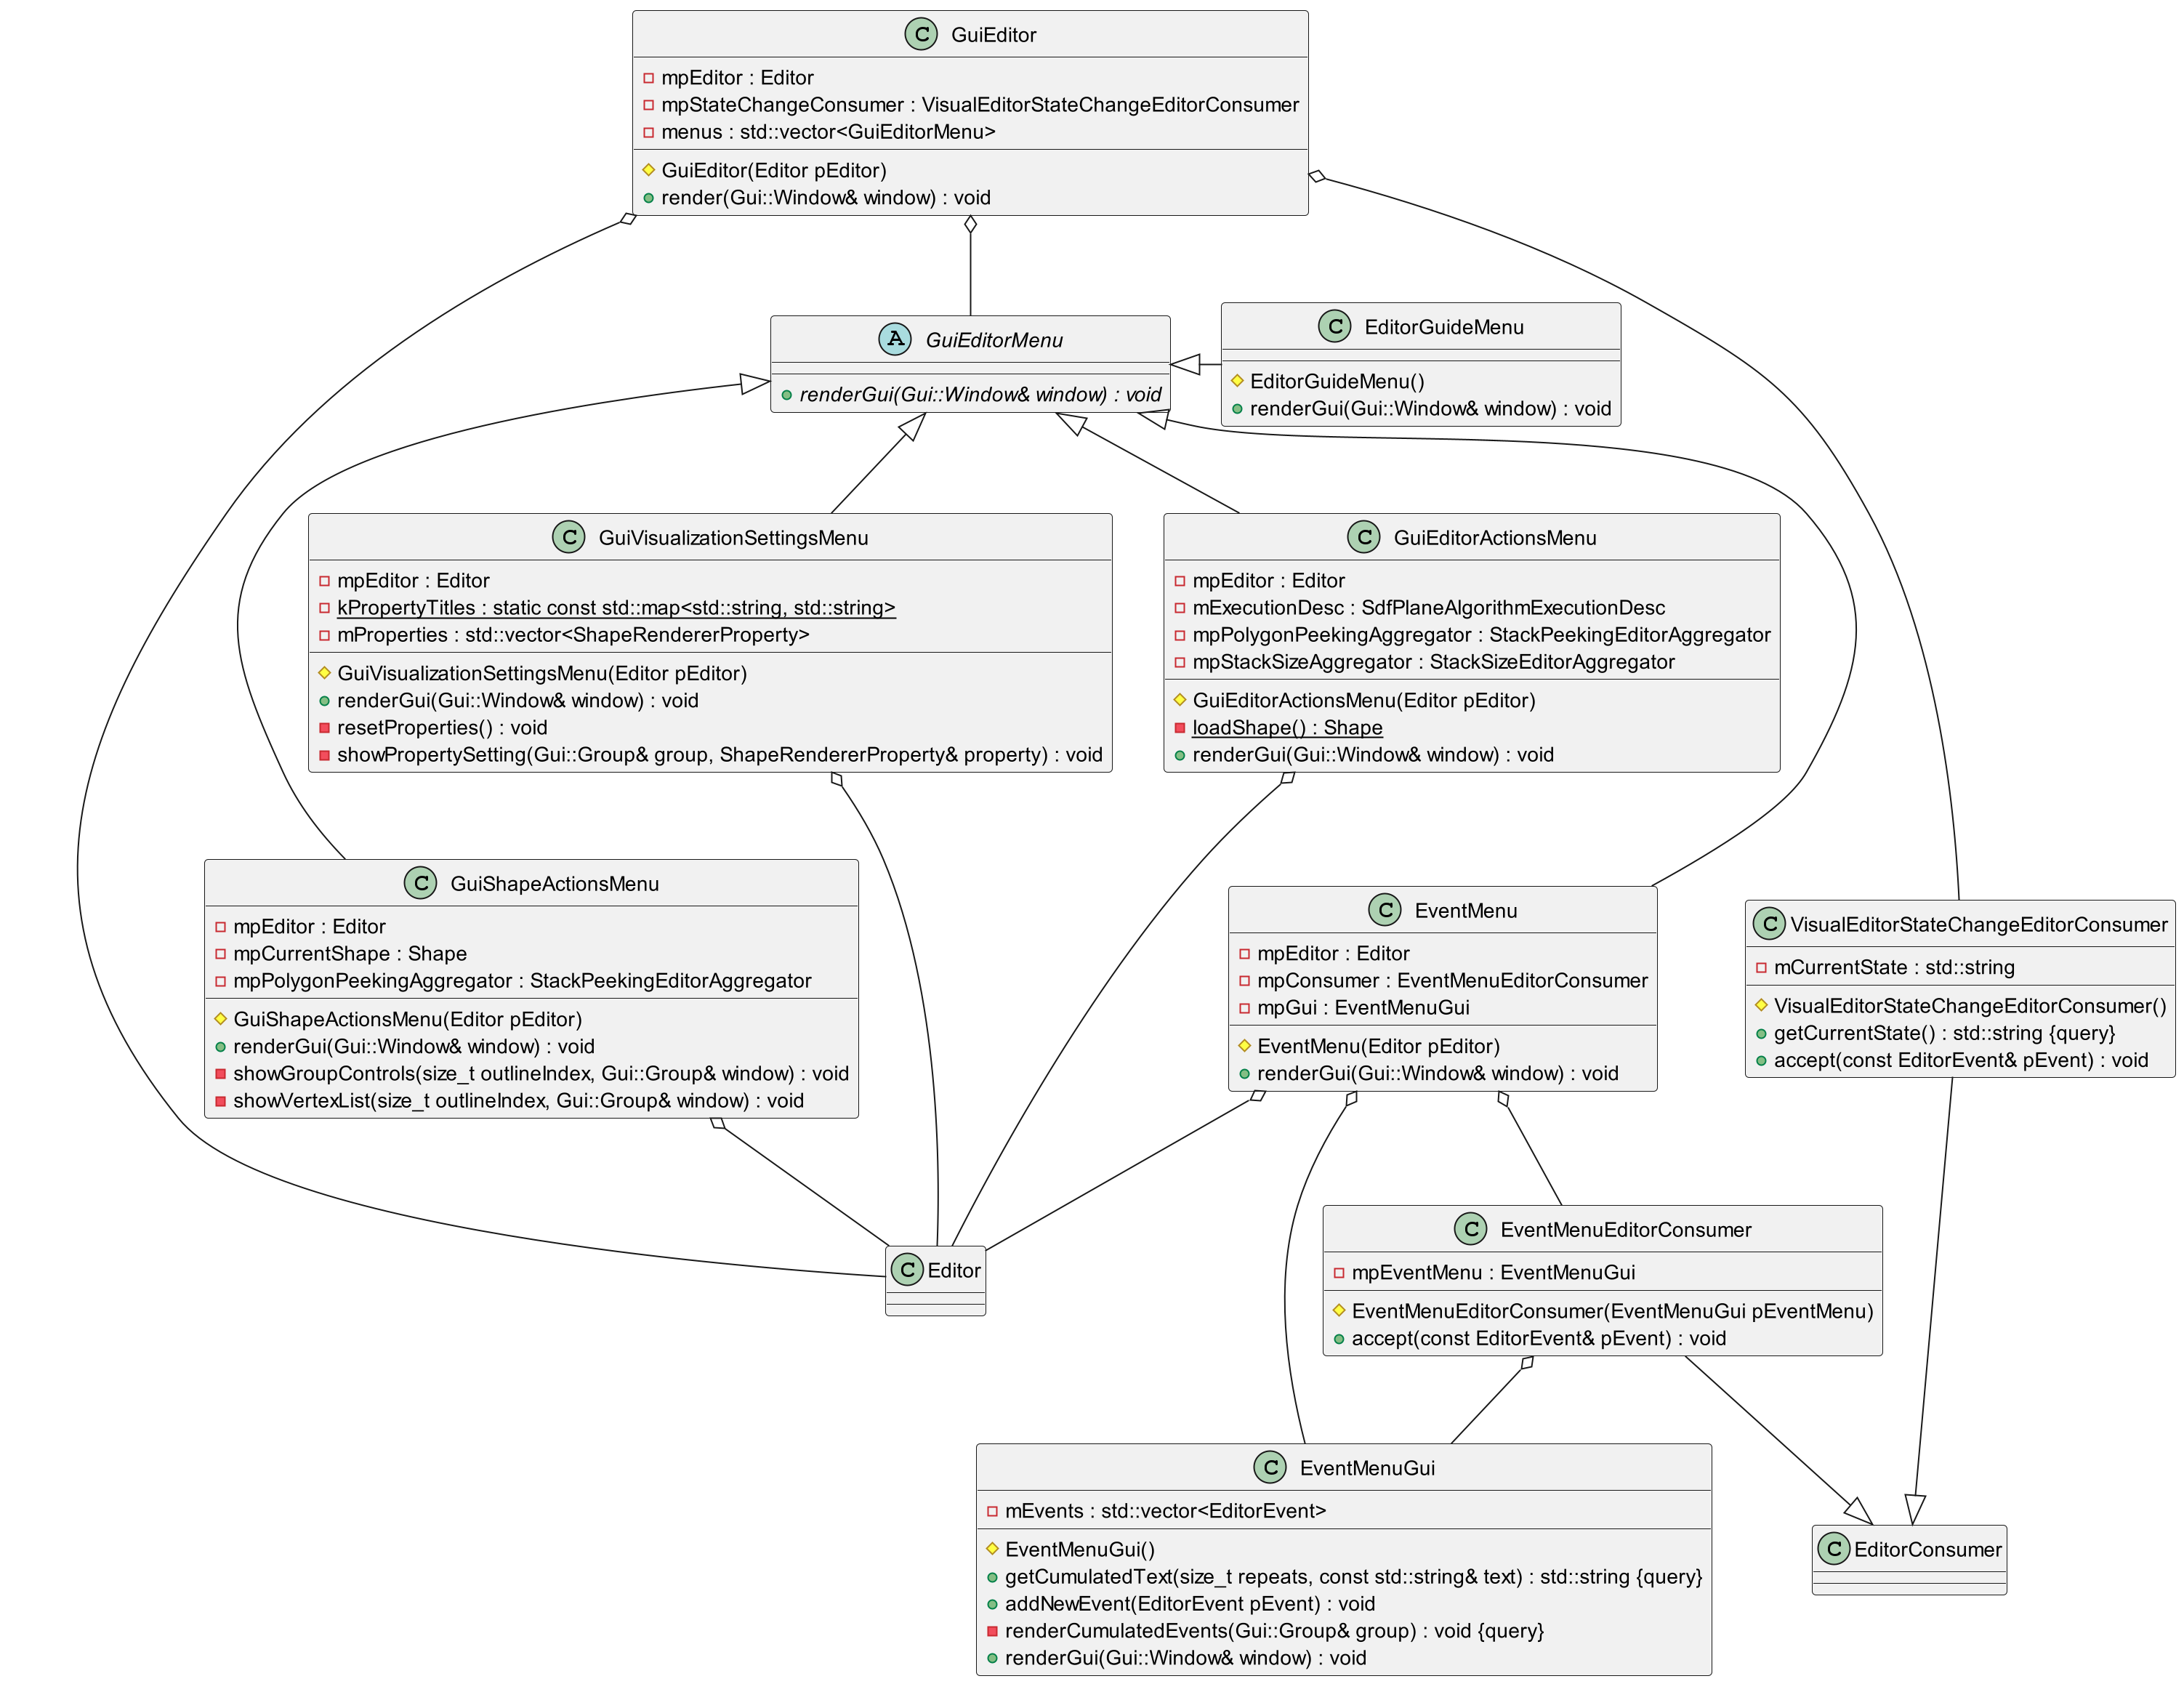
\includegraphics[width=1\linewidth]{images/class_gui_editor.png}
    \caption{A GUI szerkesztő osztálydiagramja}
    \label{fig:class_gui_editor-1}
\end{figure}

\textbf{A szerkesztői menük}

\begin{description}
    \item[GuiVisualizationSettingsMenu] -- A megjelenítési beállítások itt érhetőek el. Kezdetben minden beállítás az alap értékével rendelkezik, aminek kiolvasása egy központi helyről történik. Amikor a felhasználó egy új értéket ad meg, akkor egy üzenettel közvetíti a változásokat.
    \item[GuiEditorActionsMenu] -- Legfőképpen gombokból álló menü, elérhetővé tesz bizonyos \textbf{EditorCommand} implementációkat.
    \item[GuiShapeActionsMenu] -- Megjeleníti az alakzatot a csúcspontok pontos koordinátáival, amiket a felhasználó kézzel is átírhat. Értékmódosításkor egy új paranccsal bővül a szerkesztő.
    \item[EventMenu] -- Kettő osztály közötti kapcsolatot kezel, egyik az \textbf{EventMenuGui}, ami megjeleníti az eseményeket egy listában és az \textbf{EventMenuEditorConsumer}, ami az események rögzítéséért lett létrehozva, az \textbf{EventMenu} konstruktora iratkoztatja fel a szerkesztőre és a destruktora iratkoztatja le.
    \item[EditorGuideMenu] -- Szöveges formában megjeleníti a vizuális szerkesztő eszközeit és azok billentyűparancsait.
\end{description}


\section{Vizuális szerkesztő}

A vizuális szerkesztő tölti be az egyik legfontosabb szerepet az alkalmazásban, mivel itt történik az alakzat megjelenítése. Az eszközök között váltogatva az egérrel módosításokat végezhetünk az alakzaton. Az algoritmus kimenetének a megjelenítésért is ez a réteg felel.

\subsection{A vizuális szerkesztő felépítése}

A vizuális szerkesztő birtokolja a megjelenítésért (\textbf{ShapeRenderer}) és bemenet feldolgozásért felelős objektumokat (\textbf{MouseInputHandler}). A \textbf{Presenter} osztály a felhasználói bemenet alapján módosítja a \textbf{ShapeRenderer}-beli transzformációt, ezzel mozgatva az alakzatot a vásznon. A billentyűparancsok lekezelése viszonylag egyszerű, csak ellenőrizzük, hogy a lenyomott billentyű tartozik-e egy eszközhöz és ha igen aktívvá tesszük, ebből adódóan nem volt szükség plusz osztályok készítésére a parancsok feldolgozásához.

\begin{figure}[H]
    \centering
    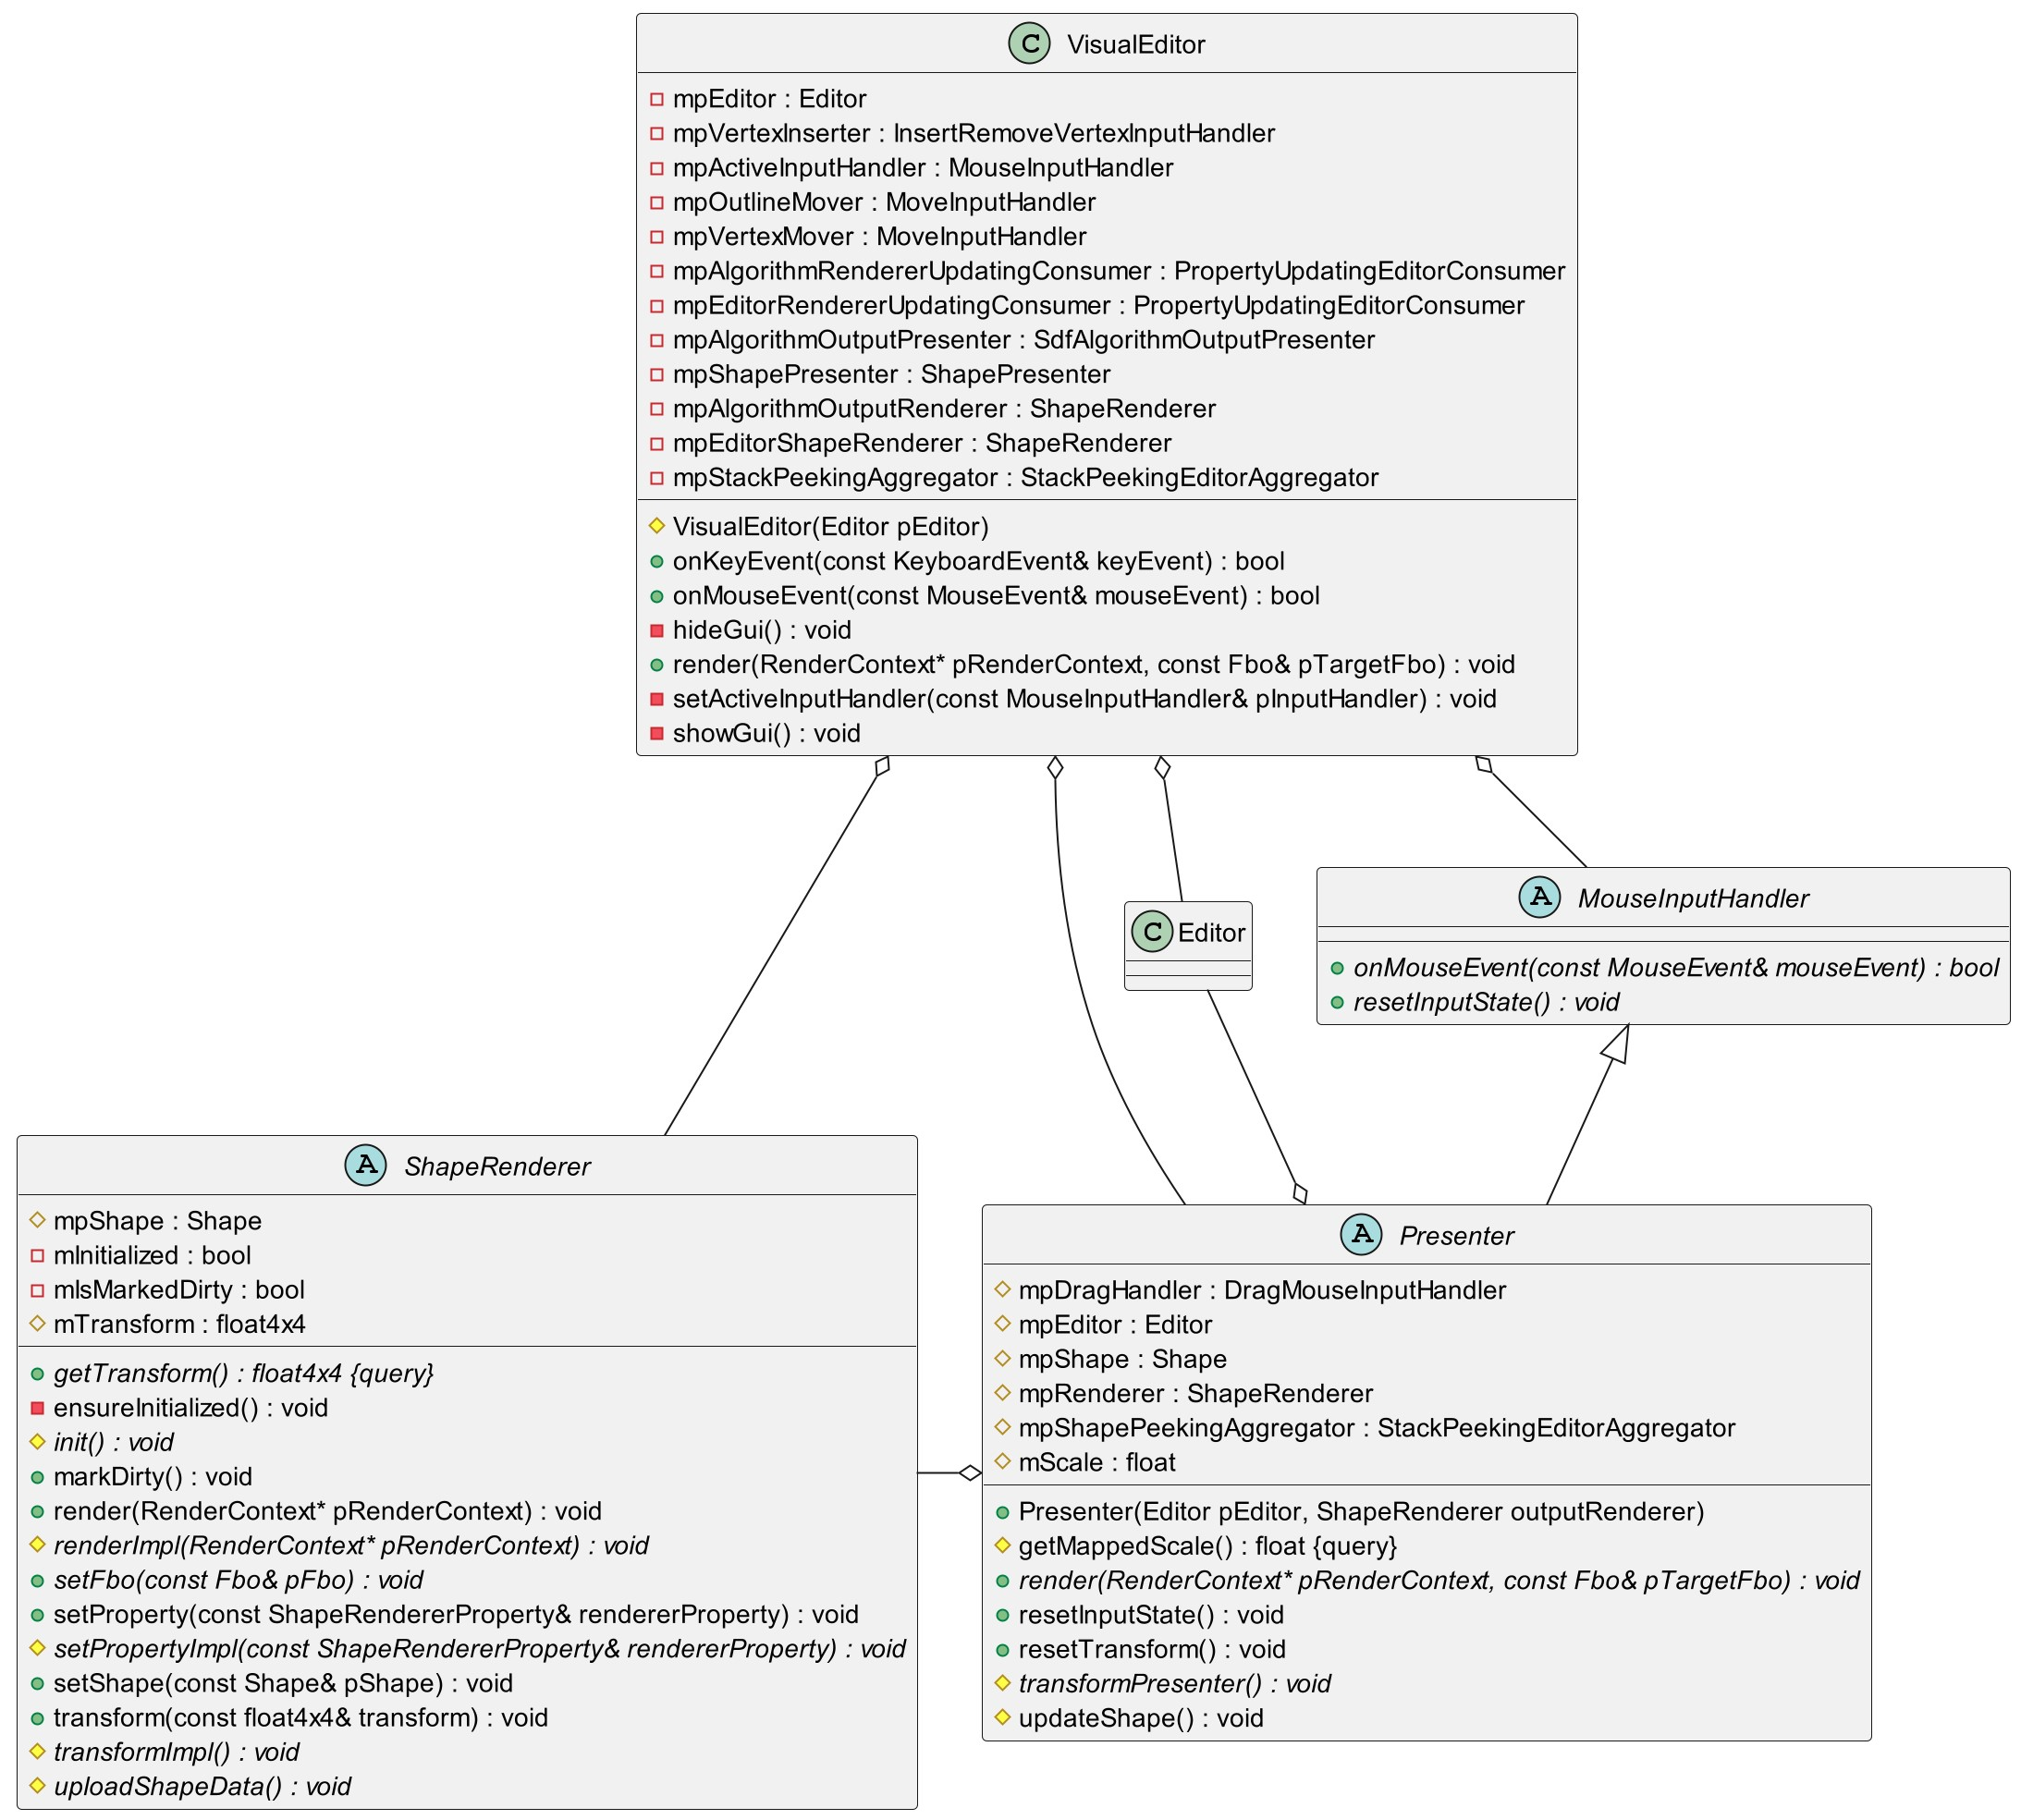
\includegraphics[width=1\linewidth]{images/class_visual_editor.png}
    \caption{A vizuális szerkesztő osztálydiagramja}
    \label{fig:class_visual_editor-1}
\end{figure}


\subsection{A MouseInputHandler osztály}

Kettő absztrakt metódussal rendelkezik, egyik az egérhez fűződő bemenet feldolgozásához (\textit{onMouseEvent}) és a több eseményt felölelő művelet (pl ,,Drag and Drop") megszakításához (\textit{resetInputState}). A felhasználói bemenet nagyon alacsony szintű információként jön be az alkalmazás osztályaiba, ezért viszonylag sok logika szükséges arra, hogy megállapítsuk, hogy milyen eseményről van szó és azt feldolgozzuk.

\begin{figure}[H]
    \centering
    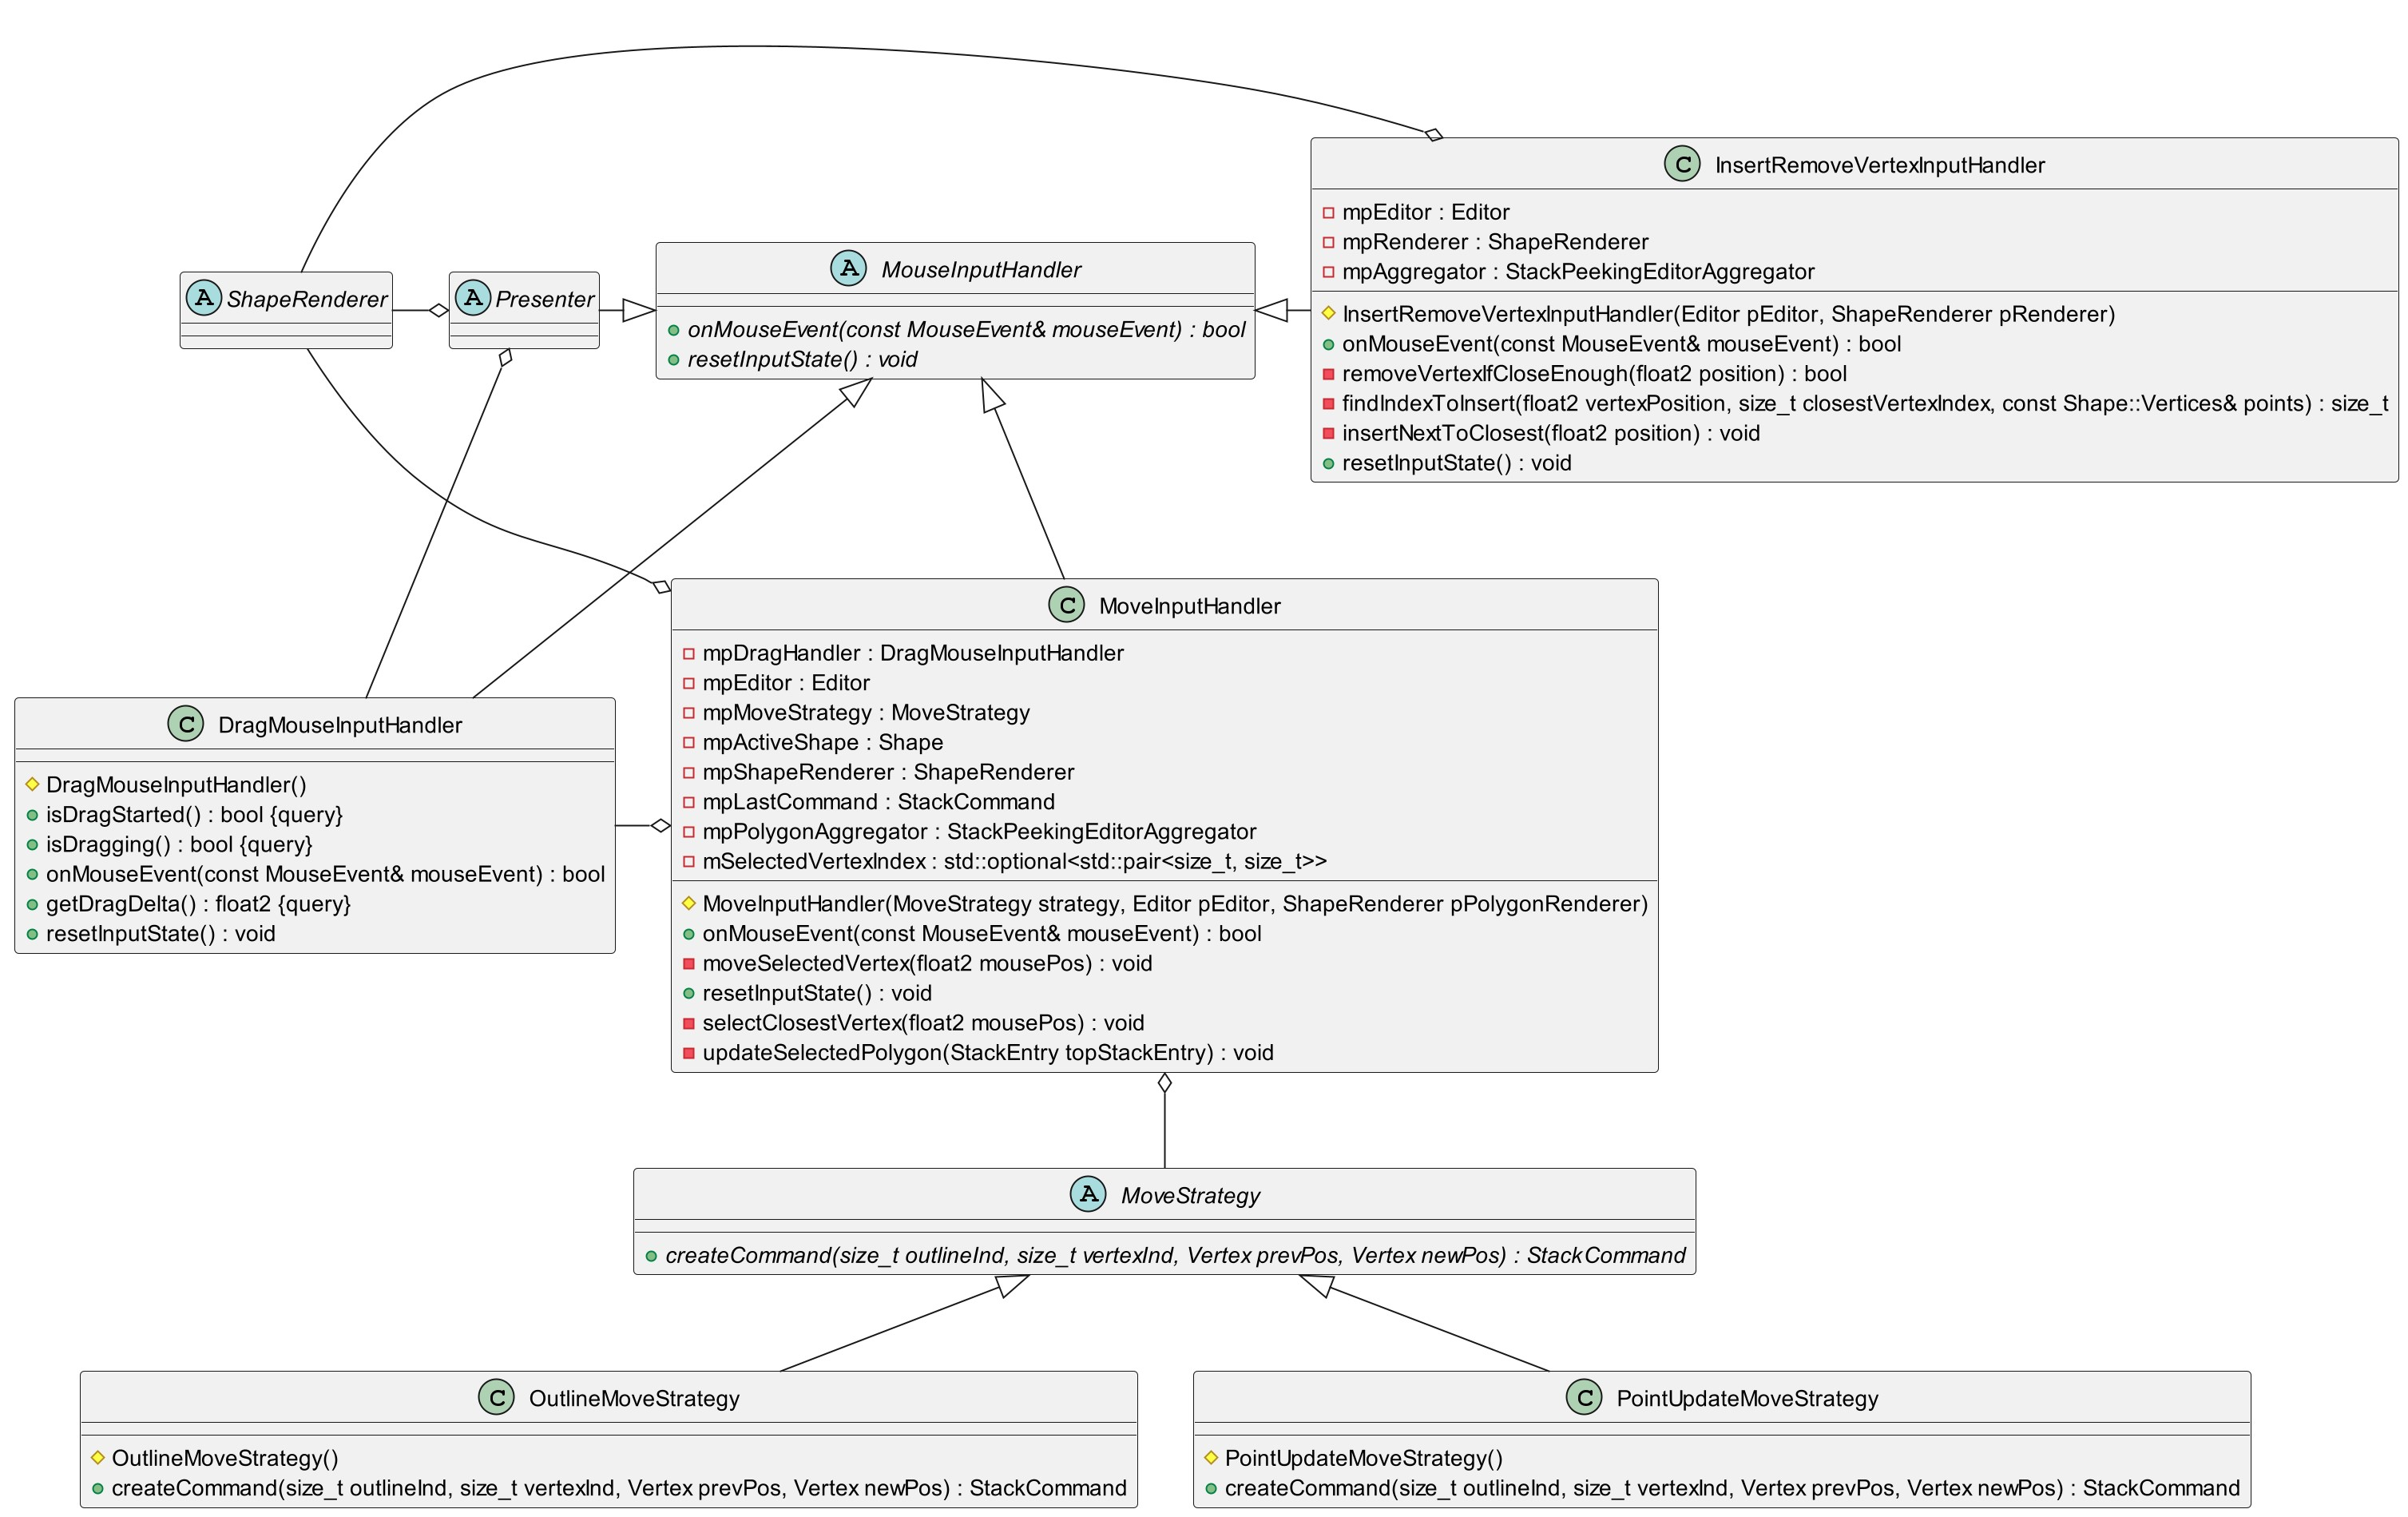
\includegraphics[width=1\linewidth]{images/class_mouse_input_handler.png}
    \caption{A MouseInputHandler osztálydiagramja}
    \label{fig:class_mouse_input_handler-1}
\end{figure}

\textbf{Az osztály implementációi/specializációi}

\begin{description}
    \item[DragMouseInputHandler] Az egérhúzást dolgozza fel, segítségével detektálhatjuk és információt nyerhetünk ki a nyers eseményadatokból. Le tudjuk kérni, hogy épp aktív-e az egérhúzás (a felhasználó nyomva tarja-e az egérgombot) és azt, hogy mennyit mozdult az egér az előző esemény óta. Az állapot visszaállításakor az aktív állapot inaktívvá válik.
    \item[InsertRemoveVertexInputHandler] Csak kattintásokra reagál. Jobb egérgomb kattintáskor megkeresi az egérhez a legközelebbi csúcspontot egy megadott korláton belül. Ha van ilyen, akkor törli. Bal kattintásra megkeresi a legközelebbi kettő csúcspontot egy poligonon belül és beszúr közéjük egy újat. Onnan tudjuk, hogy az alakzaton belül hova kattintunk, hogy a \textbf{ShapeRenderer}-ben lévő transzformációs mátrix segítségével az egér koordinátája átalakításra kerül az alakzat koordináta-rendszerébe.
    \item[MoveInputHandler] Egérhúzással mozgatja egy csúcspontot vagy egy poligont a konstruktorban megadott \textbf{MoveStrategy} alapján, a mozgatási stratégia csak a kiadott parancsot szabja meg. A mozgatás úgy történik, hogy a kattintáskor megkeresi a legközelebbi csúcspontot, ami egy megadott korláton belül van. Ha létezik ilyen, akkor az egérgomb elengedéséig mozgatáskor a csúcspont pozícióját az egér pozíciójára állítja be. A helyes pozíciók meghatározásához az egér pozíciója a \textbf{ShapeRenderer} transzformációs mátrixával az alakzat koordináta-rendszerébe kerül átszámításra.
    \item[Presenter] Az alakzat megjelenítéséért és mozgatásáért felel. A \textbf{DragMouseInputHandler} segítéségével meghatározza azt, hogy mennyit kell mozdítanunk az alakzaton a \textbf{ShapeRenderer}-en keresztül.
\end{description}

\subsection{A Presenter osztály}

Ez az osztály felel azért, hogy lefordítsa a felhasználói bemenetet transzformációkra az alakzat megjelenítésekor. A szerkesztői nézetben az egérrel mozgathatjuk a vásznon az alakzatot, a háromdimenziós nézetben pedig forgathatjuk. Mindkét nézetben a görgővel nagyíthatjuk és kicsinyíthetjük a megjelenített objektumot. Mivel a bemenet feldolgozása jelentősen eltér a két nézet esetében, ezért két implementációval rendelkezik ez az absztrakt osztály, melynek diagramját a \ref{fig:class_presenter-1}-es ábrán láthatjuk.

\begin{figure}[H]
    \centering
    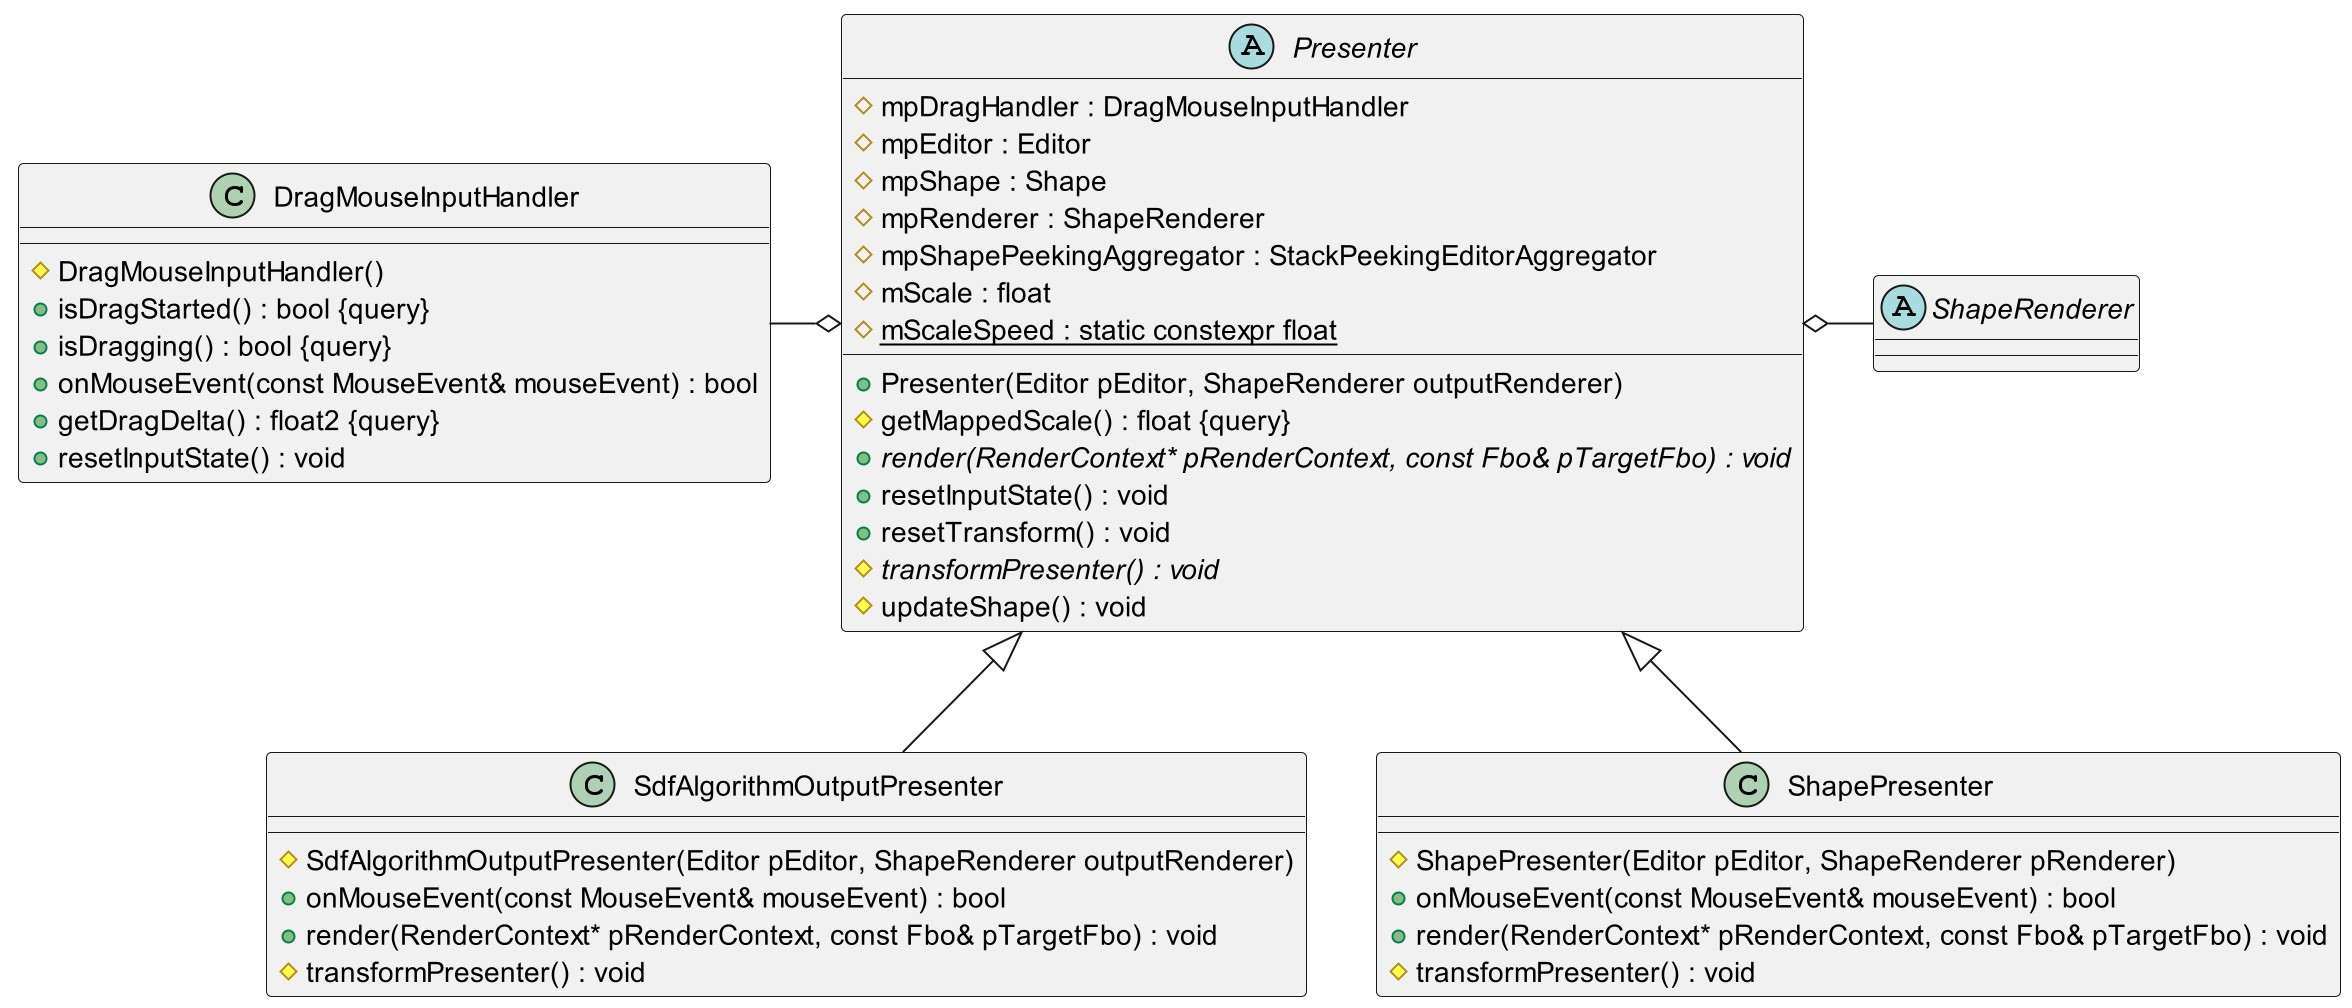
\includegraphics[width=1\linewidth]{images/class_presenter.png}
    \caption{A Presenter osztálydiagramja}
    \label{fig:class_presenter-1}
\end{figure}

\textbf{Az osztály implementációi/specializációi}

\begin{description}
    \item[ShapePresenter] A szerkesztői nézetbeli megjelenítő irányításáért felel.
    \item[SdfAlgorithmOutputPresenter] Az algoritmus kimeneteként kapott háromdimenziós objektum megjelenítése történik az osztályon keresztül.
\end{description}

\subsection{A ShapeRenderer osztály}

Ez az absztrakt osztály függvényeket biztosít egy alakzat kirajzolására egy FrameBufferbe. Az osztály implementációi lehetővé teszik, hogy több ShapeRenderer által nyújtott funkcionalitást (pl körvonal és távolságvizualizáció együttes megjelenítése) összekombináljunk a kompozit tervminta alapján. Ez mind úgy történik, hogy a felhasználó objektum nem tudja azt, hogy akár több \textbf{ShapeRenderer} is együttműködhet a háttérben akár teljesen eltérő rajzolási módszerekkel. Az összes implementáció diagramja a \ref{fig:class_shape_renderer-1}-as ábrán látható.

\begin{figure}[H]
    \centering
    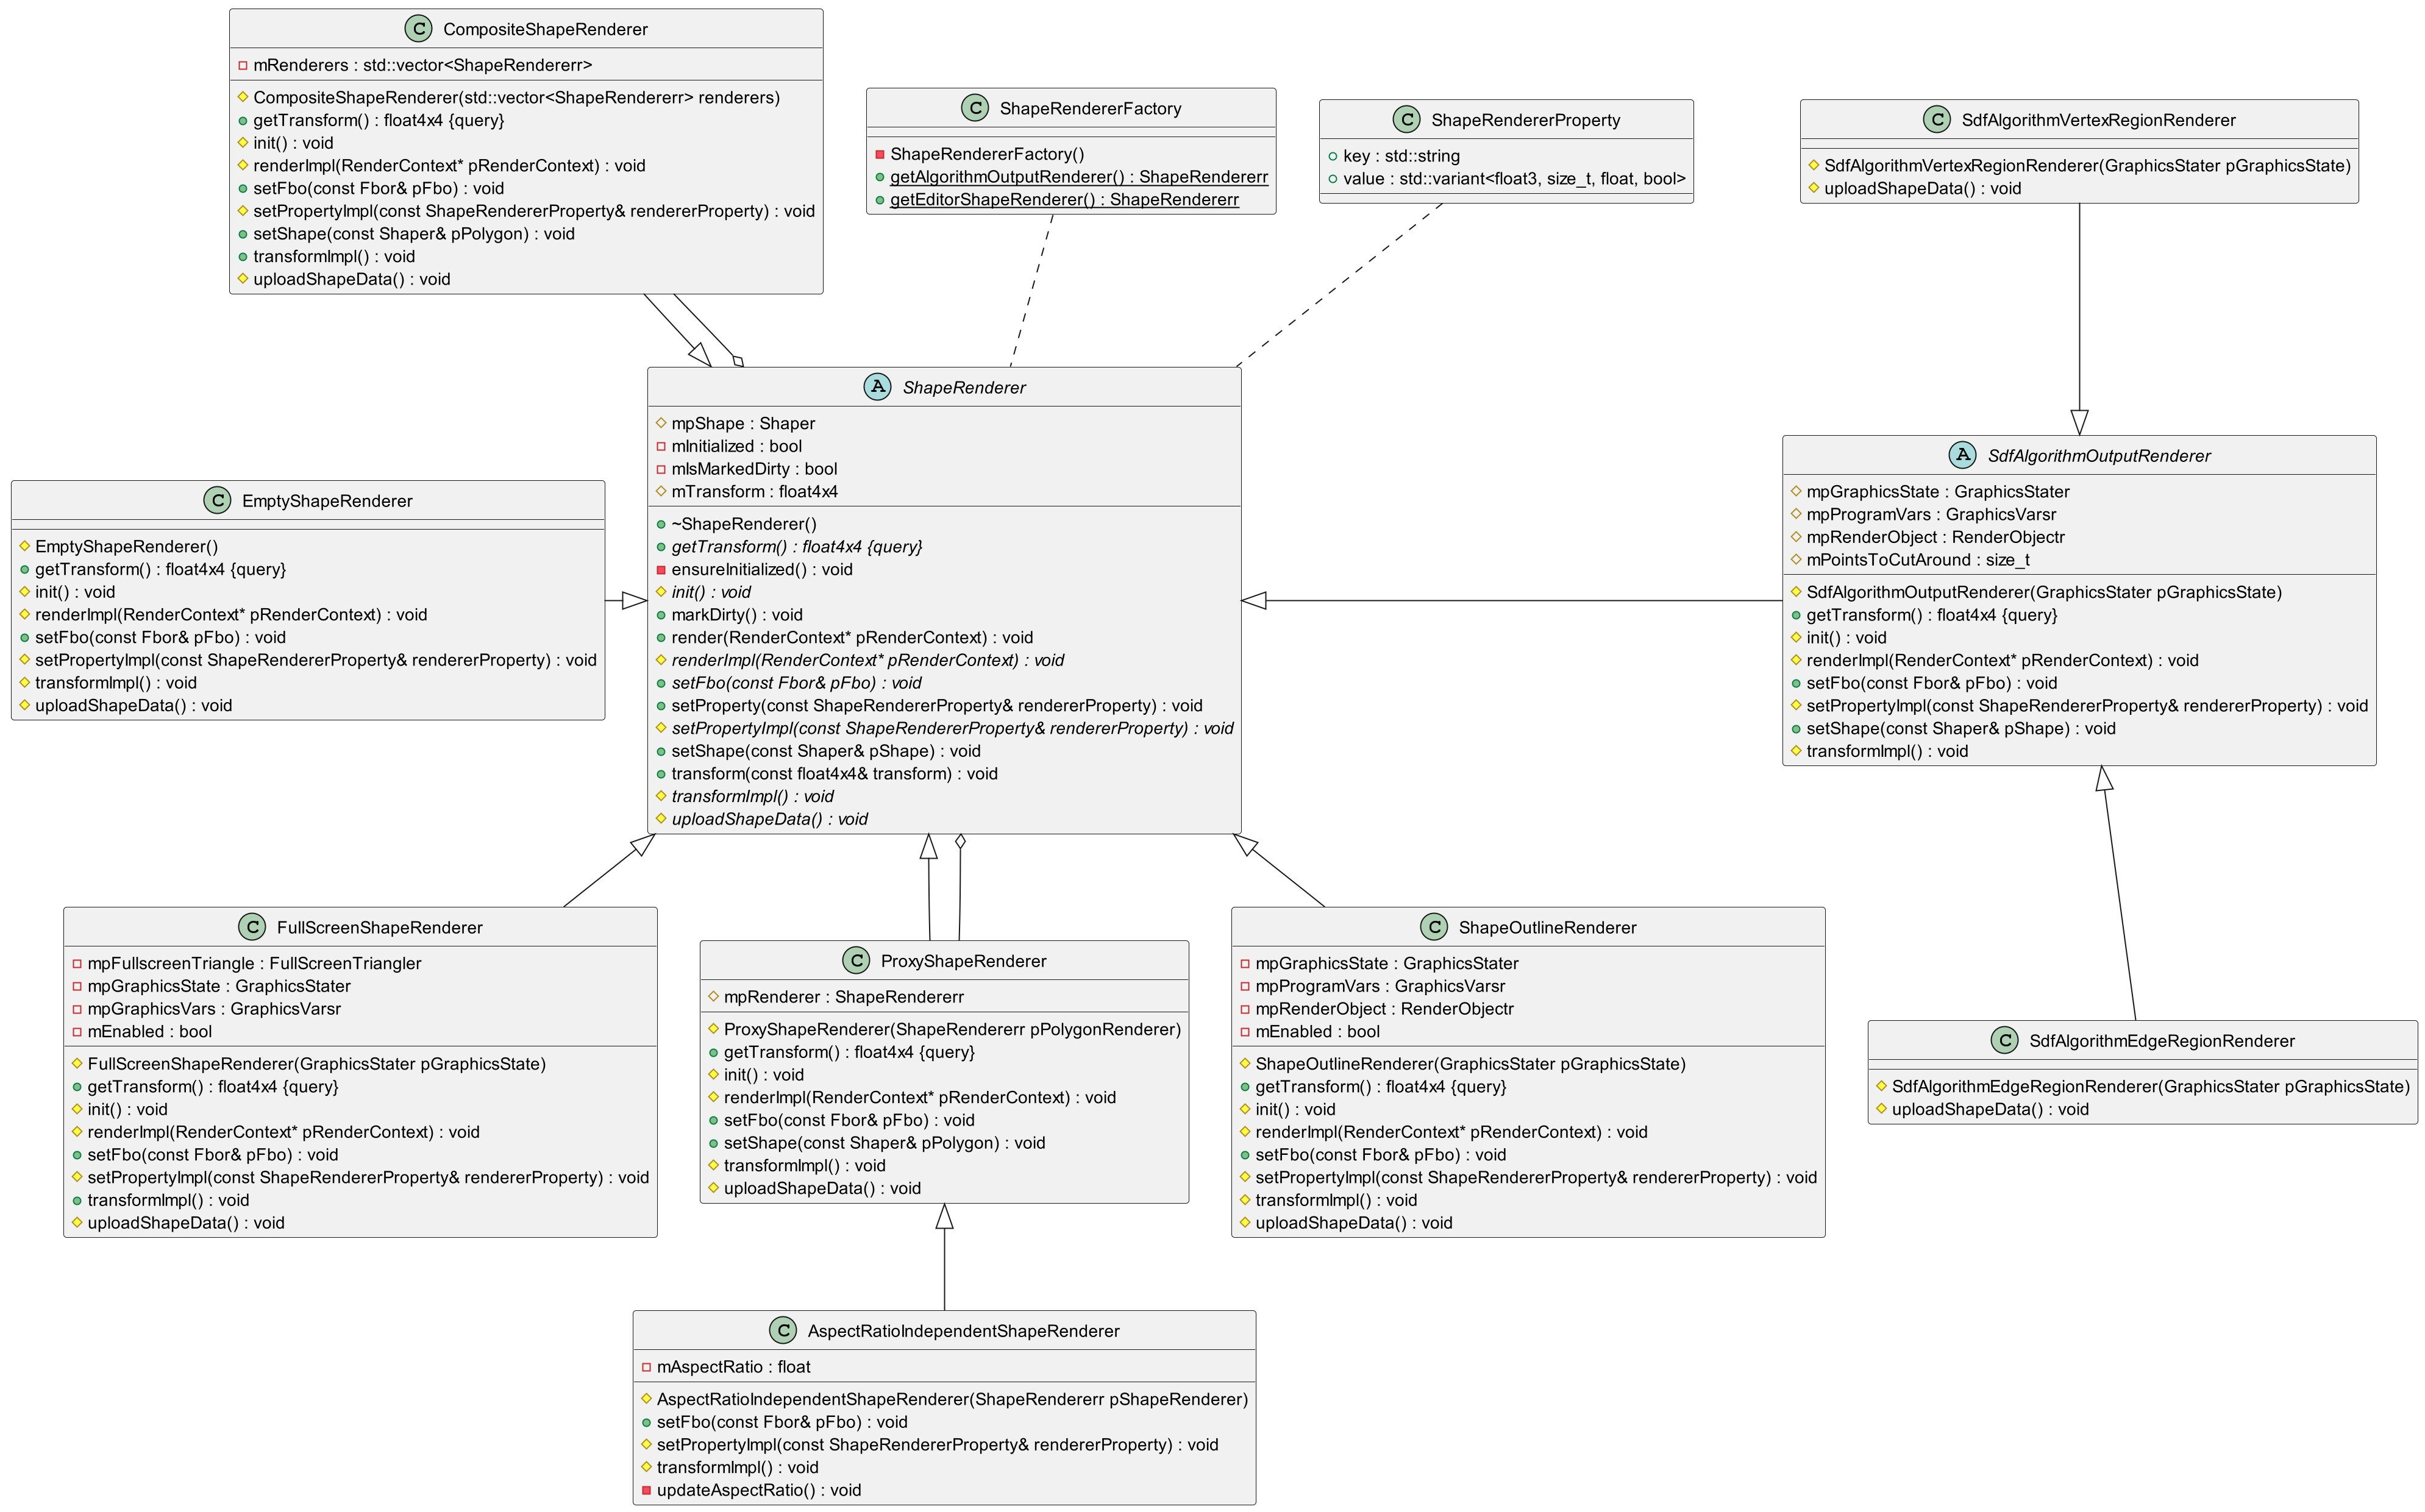
\includegraphics[width=1\linewidth]{images/class_shape_renderer.png}
    \caption{A ShapeRenderer osztálydiagramja}
    \label{fig:class_shape_renderer-1}
\end{figure}

\textbf{Az osztály implementációi/specializációi}

\begin{description}
    \item[ProxyShapeRenderer] Az osztály absztrakt, viszont minden metódusa rendelkezik implementációval, amiben a konstruktorban megkapott \textbf{ShapeRenderer} objektum metódusait delegálja. Megkönnyíti olyan implementációk készítését, amik egy meglévő objektumot befolyásolnak.
    \item[AspectRatioIndependentShapeRenderer] Egy olyan \textbf{ProxyShapeRenderer} implementáció, ami a bejövő transzformációhoz egy ortogonális kamerát ad, ami a rajzolási cél mérete alapján kerül kiszámításra. Ez a lépés nélkül a képernyő oldalarányai változásával torzulna az megjelenő objektum.
    \item[CompositeShapeRenderer] Lehetővé teszi, hogy több \textbf{ShapeRenderer} objektumot egyetlen objektum alá csoportosítsunk.
    \item[EmptyShapeRenderer] Üres metódustörzsekkel rendelkező implementáció, a tesztelésben hasznos.
    \item[FullScreenShapeRenderer] Rajzoláskor egy a teljes képernyőt kitöltő háromszögre rajzol a konstruktorban megkapott shaderrel. A szerkesztőben ez a osztály felel a távolság megjelenítéséért.
    \item[SdfAlgorithmOutputRenderer] Az algoritmus kimenetének megjelenítéséért felel. Egyetlen absztrakt metódusa van, az alakzathoz tartozó adat feltöltése a GPU memóriába (\textit{uploadShapeData}), mert a csúcsrégiók és az élrégiók esetében máshogy kell ebben a lépésben eljárni.
    \item[SdfAlgorithmEdgeRegionRenderer] Implementálja az \textbf{SdfAlgorithmOutputRenderer} absztrakt osztályt, a csúcsrégiók adatainak feltöltésével.
    \item[SdfAlgorithmVertexRegionRenderer] Implementálja az \textbf{SdfAlgorithmOutputRenderer} absztrakt osztályt, a élrégiók adatainak feltöltésével.
    \item[ShapeOutlineRenderer] Az alakzat körvonalának megjelenítéséért felel. A rajzolás a GPU-n történik.
\end{description}

\subsection{Az alakzat megjelenítése a szerkesztőben}

A szerkesztői nézet két megjelenítőt tartalmaz, egy \textbf{FullScreenShapeRenderer}-t és egy \textbf{ShapeOutlineRenderer}-t, melyeket egy \textbf{CompositeShapeRenderer} fog össze egy objektumba, amit egy \textbf{AspectRatioIndependentShapeRenderer} csomagol be, hogy a végeredmény ne függjön a képernyő oldalarányától.

A GPU-val az alkalmazás a DirectX12 API segítségével kommunikál a Falcor keretrendszer által nyújtott magasabbszintű osztályokon keresztül. A shadereket Slang-ban kell írni, amire tekinthetünk úgy, mint a HLSL egy kibővített verziója. A nyelv rendkívül jó fejlesztői élményt nyújt, a fordító tisztában van a fájlrendszerrel, ezért használhatjuk az \textit{\#include} makrót fájlok bemásolásához, támogatja a generikus típusokat és még sok más produktivitást növelő funkciót. (todo ref)

A körvonal megjelenítéséhez az textbf{ShapeOutlineRenderer} az alakzat szakaszait primitívként feltölti a GPU-ra és a paraméterként átadott shaderrel kirajzolja, a felhasználó által beállított színben.

A távolság vizualizáció esetében egy háromszöget igazítunk a képernyőre úgy, hogy azt teljesen lefedje és a háromszögben megadott UV koordináták interpolációja után a képernyő bal alsó sarkában legyen a (0,0) pont és a jobb felső sarkában az (1,1), ez az érték képviseli a számításainkban a pont pozícióját, amihez a távolságot ki szeretnénk számolni. Az UV koordináták eltolásával és skálázásával pedig szimulálhatjuk az alakzat eltolását és méretezését a képernyőn.

A fejlesztői nézetben a távolságot a naiv, lassú módszerrel vizualizáljuk, viszont az előnye az, hogy nagyon könnyen párhuzamosítható, ami fontos, ha a GPU-n egy shader formájában szeretnénk futtatni és az algoritmus működik olyan alakzatokra is amiben vannak önmetsző poligonok. Az utóbbit a szakdolgozatban implementált algoritmus nem tudja lekezelni. (todo https://www.shadertoy.com/view/wdBXRW)

A távolság értékét, ami egy lebegőpontos, negatív és pozitív értékeket is felvehető szám átszámoljuk egy színné a képernyőn a \ref{src:distance-visualization}-as kódrészlet segítségével.

\lstset{caption={Távolsági érték átszámítása színértékbe}, label=src:distance-visualization}
\begin{lstlisting}[language=c]
	cbuffer DistanceColoringSettings
	{
		float3 iPositiveColor;
		float3 iNegativeColor;
		float iContourFrequency;
		float iContourIntensity;
		bool iDisplayShadows;
		float iShadowIntensity;
		bool iDisplayCloserToVertex;
		bool iShouldDisplayContours;
		bool iShouldColorBetweenContours;
	}

	struct DistanceDesc
	{
		float distance;
		bool closerToVertex;
	};

	float4 signedDistanceToColor(DistanceDesc desc)
	{
		float distance = desc.distance;
		float3 col = (distance > 0.0)
		? iPositiveColor
		: iNegativeColor;
		col *= 1.0 - exp(-iShadowIntensity * abs(distance))
		* int(iDisplayShadows);
		float colorBetweenContours = (1 - iContourIntensity)
		* int(iShouldColorBetweenContours);
		float colorContour = iContourIntensity
		* cos(iContourFrequency * distance)
		* int(iShouldDisplayContours);
		col *= colorBetweenContours + colorContour;
		col = lerp(col,
		float3(1),
		1 - smoothstep(0, 0.01, abs(distance)));
		if (desc.closerToVertex && iDisplayCloserToVertex)
		{
			col *= .7;
		}
		return float4(col, 1);
	}

\end{lstlisting}

\subsection{Az alakzat háromdimenziós nézete}

A háromdimenziós nézet három levélszintű megjelenítőt tartalmaz, egy \textbf{SdfAlgorithmEdgeRegionRenderer}-t, egy \textbf{SdfAlgorithmVertexRegionRenderer}-t és egy \textbf{ShapeOutlineRenderer}-t, melyeket egy \textbf{CompositeShapeRenderer} fog össze egy objektumba, amit egy \textbf{AspectRatioIndependentShapeRenderer} csomagol be, hogy a végeredmény ne függjön a képernyő oldalarányától.

Annyi különlegesség van a megjelenítésében az algoritmus kimenetének a megjelenítésében, hogy a vertex shaderben a Z koordináta az előjeles távolság abszolút értéke lesz, csúcsrégiókhoz tartozó geometria esetében pedig a pixel shaderben is felülírjuk az interpolált mélységet a távolság abszolút értékével, a csúcsrégiók pixel shaderét (\textit{psMain}) a \ref{src:vertex-region-shader}-es kódrészletben láthatjuk. A \ref{src:edge-region-shader}-ös kódrészletben láthatjuk az élrégiók vertex shaderét (\textit{vsMain}) és pixel shaderét (\textit{psMain}).

\lstset{caption={Csúcsrégiók raszterizálásának vertex és pixel shadere}, label=src:vertex-region-shader}
\begin{lstlisting}[language=c]
	#include "DistanceVisualization.slang"

	cbuffer Data
	{
		float4x4 iTransform;
	}

	struct VsIn
	{
		float2 regionVertex : RV;
		float2 vertexPos : POS;
		float signedDistance : DST;
	};

	struct VsOut
	{
		nointerpolation float2 regionVertex : RV;
		float2 samplePos : POS;
		float4 vertexPos : SV_POSITION;
		float signedDistance : DST;
	};

	struct PsOut
	{
		float4 color : SV_TARGET;
		float depth : SV_DEPTH;
	};

	VsOut vsMain(VsIn input)
	{
		VsOut vsOut;
		vsOut.vertexPos = mul(iTransform,
		float4(input.vertexPos, abs(input.signedDistance), 1));
		vsOut.signedDistance = input.signedDistance;
		vsOut.regionVertex = input.regionVertex;
		vsOut.samplePos = input.vertexPos;
		return vsOut;
	}

	PsOut psMain(VsOut vsOut, uint triangleIndex : SV_PrimitiveID)
	: SV_TARGET
	{
		DistanceDesc desc;
		float dst = distance(vsOut.regionVertex, vsOut.samplePos);
		desc.distance = dst * sign(vsOut.signedDistance);
		desc.closerToVertex = false;

		PsOut psOut;
		psOut.color = signedDistanceToColor(desc);
		psOut.depth = dst;
		return psOut;
	}
\end{lstlisting}


\lstset{caption={Élrégiók raszterizálásának vertex és pixel shadere}, label=src:edge-region-shader}
\begin{lstlisting}[language=c]
	#include "DistanceVisualization.slang"

	cbuffer Data
	{
		float4x4 iTransform;
	}

	struct VsIn
	{
		float2 vertexPos : POS;
		float signedDistance : DST;
	};

	struct VsOut
	{
		float4 vertexPos : SV_POSITION;
		float signedDistance : DST;
	};

	struct PsOut
	{
		float4 color : SV_TARGET;
		float depth : SV_DEPTH;
	};

	VsOut vsMain(VsIn input)
	{
		VsOut vsOut;
		vsOut.vertexPos = mul(iTransform,
		float4(input.vertexPos, abs(input.signedDistance), 1));
		vsOut.signedDistance = input.signedDistance;
		return vsOut;
	}

	PsOut psMain(VsOut vsOut, uint triangleIndex : SV_PrimitiveID)
	: SV_TARGET
	{
		DistanceDesc desc;
		desc.closerToVertex = true;
		desc.distance = vsOut.signedDistance;

		PsOut psOut;
		psOut.color = signedDistanceToColor(desc);
		psOut.depth = vsOut.signedDistance;
		return psOut;
	}
\end{lstlisting}


\section{Perzisztencia}

Az alakzatok írhatóak és olvashatóak a fájlrendszerbből. Amennyiben a szerkesztő jelenlegi alakzatára végre van hajtva az algoritmus, az is lementhető.

Minden adat szerializációja JSON formátumba történik, melynek számos előnye van, például széleskörűen elterjedt és könnyű olvashatóság az ember számára.

\subsection{Alakzat szerializációja}

Az alakzatok menthetőek és betölthetőek. Olvasáskor az alkalmazásban nem csak séma validáció történik, hanem ellenőrzésre kerül az is, hogy a beolvasott alakzat helyes-e, rendelkezik-e legalább egy poligonnal és minden poligon rendelkezik-e legalább három csúccsal. Az alakzat JSON sémája a \ref{src:shape-json-schema}-os kódrészletben látható.

\lstset{caption={Alakzat JSON sémája}, label=src:shape-json-schema}
\begin{lstlisting}[language=C]
	type Shape = {
		outlines: Outline[]
	}

	type Outline = Point[]

	type Point = {
		x: number,
		y: number
	}
\end{lstlisting}


\subsection{Algoritmus kimenetének szerializációja}
Az algoritmus kimenetét le lehet menteni a fájlrendszerbe JSON formátumban. Az algoritmus kimenetében az alakzat összes csúcspontja és éle is benne van, mivel annak raszterizáláshoz arra az információra is szükségünk van. Az algoritmus kimenetének JSON sémája a \ref{src:algorithm-output-json-schema}-es kódrészletben látható.

\lstset{caption={Algoritmus kimenetének JSON sémája}, label=src:algorithm-output-json-schema}
\begin{lstlisting}[language=C]
	type AlgorithmOutput = {
		edgeRegions: EdgeRegion[],
		vertexRegions: VertexRegion[]
	}

	type EdgeRegion = {
		bounds: Vertex[],
		start: Vertex,
		end: Vertex
	}

	type VertexRegion = {
		bounds: Vertex[],
		vertex: Vertex,
		cornerSign: number
	}

	type Vertex = {
		x: number,
		y: number
	}
\end{lstlisting}


\section{Tesztelés}

A szoftver világában a tesztelés az, amivel időtállóvá tehetünk egy kódbázist, mert segít felismerni, ha egy változtatással valami meglévő funkcionalitást módosítottunk. Mivel a tesztekkel a kód viselkedését is validáljuk, ezért remek eszköz a kód megismerésére is, az elvárt kimenetek értelmezésével, bemutatásra kerül az is, hogy egy osztályt hogy kell használni, így példaként is kezelhető.
Az alkalmazásban az algoritmus és a szerkesztő került tesztelésre.

\subsection{Az algoritmus tesztelése}

Az algoritmus tesztelése szinten történt, függvények szintjéről kiindulva egészen egy teljes alakzaton való végrehajtásig. Minden tesztesethez bemeneti fájlok tartoztak, melyekre végrehajtásra került az adott számítás, majd az elvárt kimenetet tartalmazó fájlokkal kerültek összehasonlításra. Ha a kimenet és a tartalom egyezik, akkor a teszt sikeres.

\textbf{Tesztelt funkcionalitás}

\begin{itemize}
    \item Csúcs - csúcs vágás -- Régióhatárok kerültek ellenőrzésre
    \item Csúcs - él vágás
    \item Él - csúcs vágás
    \item Él - él vágás
    \item Az algoritmus végrehajtása teljes alakzatra
\end{itemize}


\subsection{A szerkesztő tesztelése}

A szerkesztő osztály teljes funkcionalitása tesztelésre került és minden az abban használt interfészek összes implementációja. A tesztek egy friss szerkesztő objektummal lépnek interakcióba egy adott funkcionalitás teszteléséhez.

\textbf{Tesztelt funkcionalitás}

\begin{itemize}
    \item \textbf{Editor} és \textbf{EditorStack} osztályok -- Állapotátmenet kezelése
    \item \textbf{EditorAggregator} implementációk
    \begin{itemize}
        \item \textbf{StackPeekingEditorAggregator} -- Kiértékelés üres és egy általános veremre.
        \item \textbf{StackSizeEditorAggregator} -- Kiértékelés üres és egy általános veremre.
    \end{itemize}
    \item \textbf{EditorCommand} implementációk
    \begin{itemize}
        \item \textbf{AddNewOutlineStackCommand} -- Poligon hozzáadása egy alakzathoz.
        \item \textbf{AddVertexStackCommand} -- Csúcspont hozzáadása egy poligonhoz.
        \item \textbf{CalculateSdfPlaneAlgorithmCommand} -- Átmegy a teszt, ha az algoritmus kiszámításra kerül.
        \item \textbf{DeleteOutlineStackCommand} -- Poligon törlése egy alakzatból.
        \item \textbf{DeleteVertexStackCommand} -- Csúcs törlése egy poligonból.
        \item \textbf{InsertVertexStackCommand} -- Csúcs beszúrása egy poligonba, egy adott pozícióra.
        \item \textbf{MergeShapeWithOffsetStackCommand} -- Két alakzat egyesítése.
        \item \textbf{SetShapeStackCommand} -- Alakzat lecserélése.
        \item \textbf{UpdateVertexStackCommand} -- Megadott poligonban, egy adott csúcs értékének módosítása.
    \end{itemize}
    \item \textbf{EditorConstraint} implementációk
    \begin{itemize}
        \item \textbf{DeleteOutlineEditorConstraint} -- Poligon törlésének letiltása, ha a művelet helytelen állapotba helyezi az alakzatot.
        \item \textbf{DeleteVertexEditorConstraint} -- Csúcs törlésének letiltása, ha a művelet helytelen állapotba helyezi a poligont.
        \item \textbf{SdfPlaneAlgorithmConstraint} -- Algoritmus végrehajtásának letiltása, ha vannak egymást metsző élek az alakzatban.
    \end{itemize}
    \item \textbf{EditorConsumer} implementációk
    \begin{itemize}
        \item \textbf{GuiStateEditorConsumer} -- Állapot váltása \textbf{ShowGuiPublishedEvent} üzenet és \textbf{HideGuiPublishedEvent} üzenet küldésekor.
        \item \textbf{PropertyUpdatingEditorConsumer} -- Tulajdonság frissítése egy \textbf{ShapeRendererben}, ha \textbf{RendererPropertyPublishedEvent} típusú üzenet kerül kiváltásra.
        \item \textbf{VisualEditorStateChangeEditorConsumer} -- Számon tartott állapot frissítése, \textbf{VisualEditorModeChangedPublishedEvent} üzenet küldésekor.
    \end{itemize}
    \item \textbf{EditorEvent} implementációk
    \begin{itemize}
        \item \textbf{ConstraintViolationEvent} -- Kiváltódás sérülő megszorítás esetén
        \item \textbf{NewStackCommandEvent} -- Kiváltódás sikeres átmenet esetén..
        \item \textbf{StackTransformedEvent} -- Kiváltódás szerkesztői transzformáció végbemenetekor.
        \item \textbf{DeleteOutlineStackCommand} -- Kiváltódás feldolgozhatatlan \textbf{EditorCommand} implementáció esetében.
    \end{itemize}
    \item \textbf{EditorTransformation} implementációk
    \begin{itemize}
        \item \textbf{ClearHistoryEditorTransformation} -- Szerkesztői előzmények törlése.
        \item \textbf{TestUndoEditorTransformation} -- Visszalépés.
    \end{itemize}
\end{itemize}

\subsection{Teljesítmény tesztek}

A grafikailag intenzív alkalmazásokban a teljesítmény kritikus szerepet játszik, mivel a legtöbb esetben valós időben kell képeket előállítani a felhasználónak, amire csak kicsivel több mint egy tucatnyi milliszekundum áll rendelkezésre. Igaz, az algoritmus nem értékelődik ki minden képkocka kirajzolásánál, sőt, a program futása alatt nagyon kevés alkalommal, viszont a felhasználói élmény érdekében fontos, hogy minél gyorsabban eredményt kapjunk.

Az algoritmust több méretű alakzattal, több csúcsrégió parabola felosztási szinttel is teszteltem, minden konfigurációt száz iteráción keresztül. A szakdolgozat készítésekor rendelkezésre állt egy MatLabos implementációja is az algoritmusnak, a teljesítmény tesztekben az ott mért időket használom majd alapvonalként.

\begin{table}[H]
    \centering
    \begin{tabular}{ | m{0.2\linewidth} | m{0.2\linewidth} | m{0.2\linewidth} | m{0.2\linewidth} | }
        \hline
        \textbf{Csúcspontok} & \textbf{Felosztások}  & \textbf{Saját idő}  & \textbf{Referencia idő} \\
        \hline \hline
        228 & 3 & 11ms & 2326ms \\
        \hline
        228 & 10 & 31ms & 2675ms \\
        \hline
        228 & 25 & 88ms & 2631ms \\
        \hline
        228 & 50 & 216ms & 1468ms \\
        \hline
        431 & 3 & 35ms & 8134ms \\
        \hline
        431 & 10 & 108ms & 8440ms \\
        \hline
        431 & 25 & 301ms & 9244ms \\
        \hline
        431 & 50 & 742ms & 4789ms \\
        \hline
        2001 & 3 & 601ms & 199485ms \\
        \hline
        2001 & 10 & 2237ms & 205704ms \\
        \hline
        2001 & 25 & 6781ms & 230432ms \\
        \hline
        2001 & 50 & 16370ms & 133285ms \\
        \hline
    \end{tabular}
    \caption{A teljesítménytesztek eredményei}
    \label{tab:benchmarks}
\end{table}
